\chapter{Oscillation Probability Calculation}
\label{chap:OscillationProbability}

It is important to understand how and where the sensitivity to the oscillation parameters comes from for both atmospheric and beam samples. An overview of how these samples respond to changes in \quickmath{\delta_{CP}}, \quickmath{\Delta m^{2}_{32}}, and \quickmath{\sin^{2}(\theta_{23})} is given in \autoref{sec:Oscillation_Overview}. This section also explains the additional complexities involved when performing an atmospheric neutrino analysis as compared to a beam-only analysis.

Without additional techniques, atmospheric sub-GeV upward-going neutrinos (\quickmath{E_{\nu} < 1.33\text{GeV}, \cos(\theta_{Z})<0.}) can artificially inflate the sensitivity to \quickmath{\delta_{CP}},zaza due to the quickly varying oscillation probability in this region. Therefore, a ``sub-sampling'' approach has been developed to reduce these biases ensuring accurate and reliable sensitivity measurements. This technique ensures that small-scale unresolvable features of the oscillation probability have been averaged over whilst the large-scale features in the oscillation probability are unaffected. The documentation and validation of this technique are found in \autoref{sec:Oscillation_FastOscillations}. The oscillation probability calculation is computationally intensive due to the large number of matrix multiplications needed. Consequently, the \texttt{CUDAProb3} implementation choice made within the fitting framework, as detailed in \autoref{sec:Oscillation_CalculationEngine}, ensures that the analysis can be done in a timely manner.

Whilst the beam neutrinos are assumed to propagate through a constant density slab of material, the density variations through the Earth result in more complex oscillation patterns for atmospheric neutrinos. Furthermore, the uncertainty in the electron density can modify the oscillation probability for the denser core layers of the Earth. The model of the Earth used within this analysis is detailed in \autoref{sec:Oscillation_MatterDensity}. This includes information about the official SK-only methodology as well as improvements that have been made to remove some of the approximations used in that analysis. Another complexity of atmospheric neutrino oscillation studies is that the height of production in the atmosphere is not known on an event-by-event basis. An analytical averaging technique that approximates the uncertainty of the oscillation probability has been followed, with the author of this thesis being responsible for the implementation and validation. This implementation of an external technique is described in \autoref{sec:Oscillation_ProdHAvergaing}.

\section{Treatment of Fast Oscillations}
\label{sec:Oscillation_FastOscillations}

As shown in \autoref{fig:Oscillation_SK_FastOscillogram}, atmospheric neutrino oscillations have a significantly more complex structure for upgoing neutrinos with energy below \quickmath{1\text{GeV}}. This is because the \quickmath{L/E} dependence of the oscillation probability in this region induces rapid variations for small changes in \quickmath{L} or \quickmath{E}. As discussed in \autoref{sec:Oscillation_Overview}, this is also the region in which atmospheric neutrinos have sensitivity to \quickmath{\delta_{CP}}. In practice, the direction of the neutrino is inferred from the direction of the final state particles traveling in the detector. The correlation between these two directions can be particularly weak for low-energy neutrino interactions. This creates a distinct difference from the beam neutrinos where the position of the source is very precisely known.

As a consequence of the unresolvable structure, an event rate consistent with the averaged oscillation probability is observed in the subGeV upgoing region. This creates a computational problem: A significantly large amount of Monte Carlo statistics would be required to accurately predict the number of events if Monte Carlo averaging was the only technique used. This section describes the `sub-sampling' approach developed for this analysis and compares it to the methodology used within the SK-only analysis.

\begin{figure}[h]
  \begin{subfigure}[t]{0.8\textwidth}
    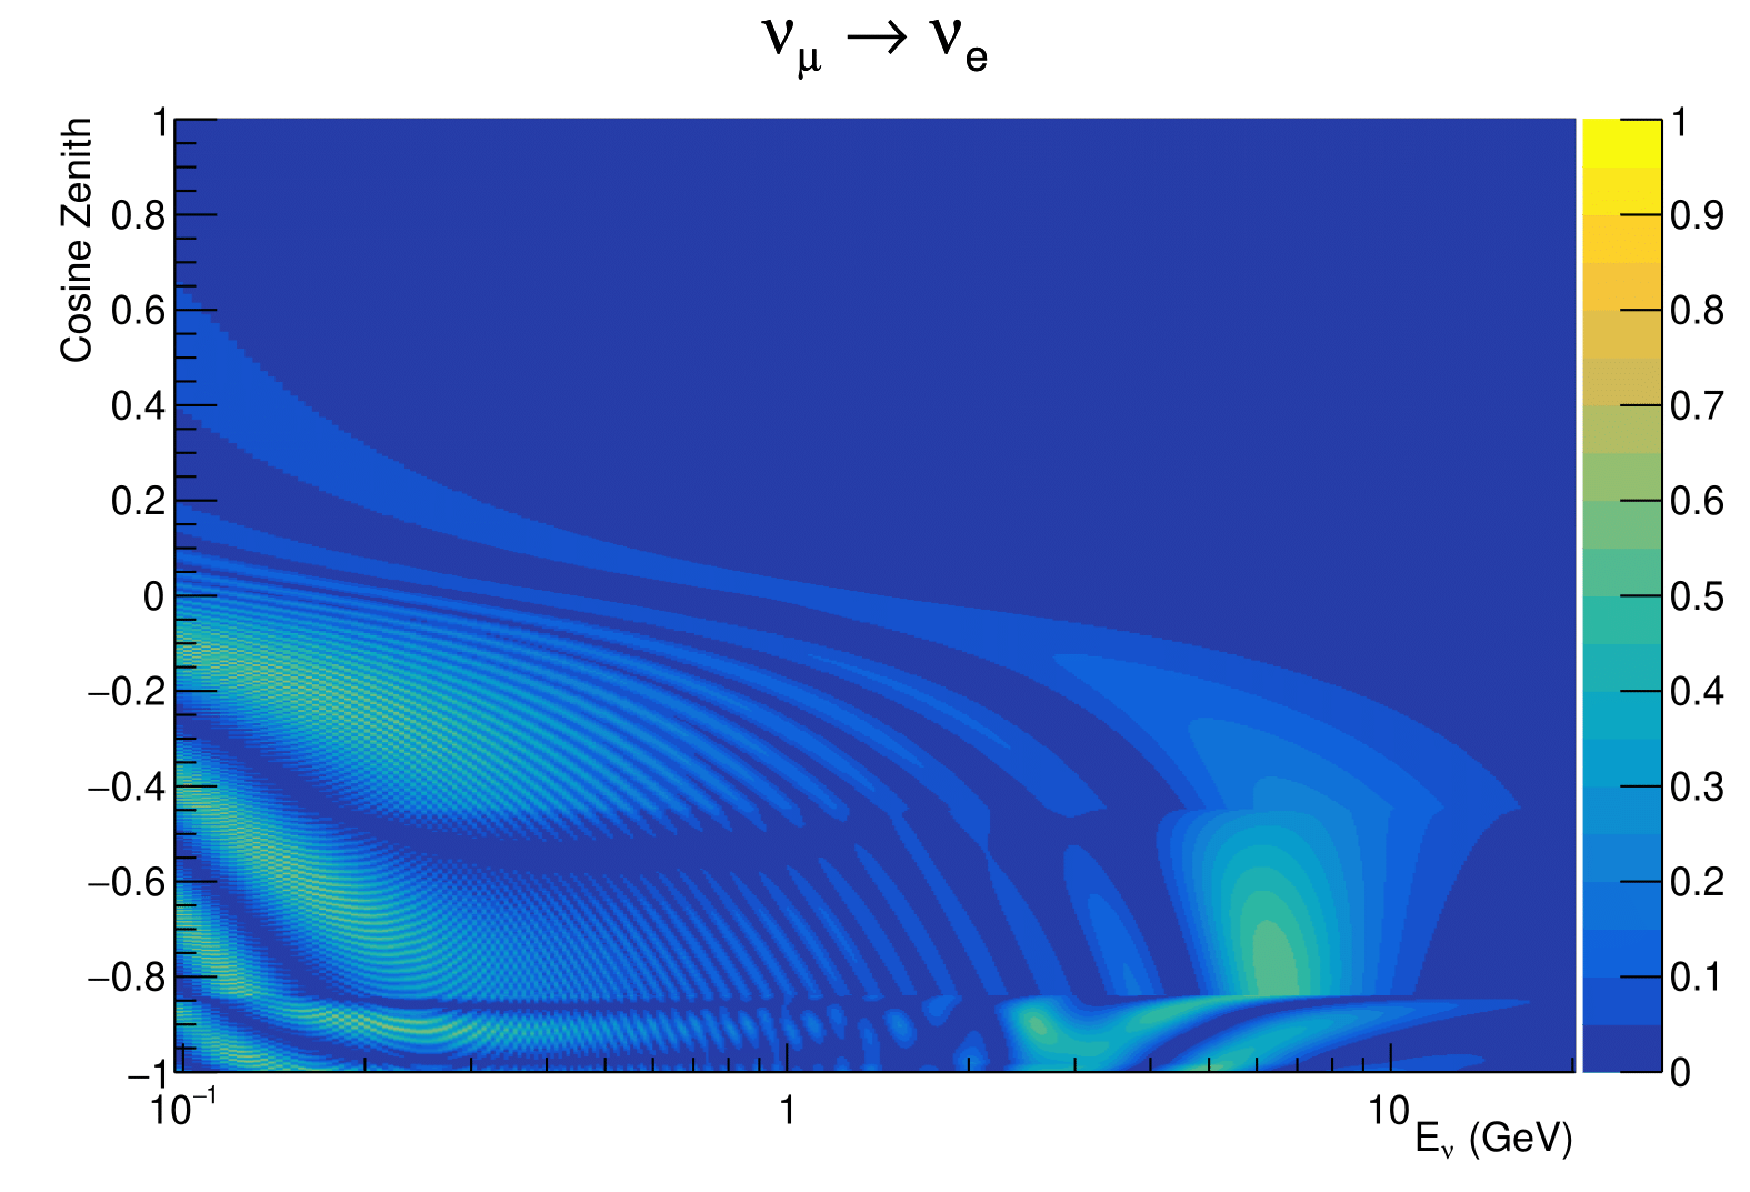
\includegraphics[width=\textwidth, trim={0mm 0mm 0mm 0mm}, clip,page=1]{Figures/Oscillation/FastOscillationExample.pdf}
  \end{subfigure}
  \caption{The oscillation probability \quickmath{P(\nu_{\mu} \rightarrow \nu_{e})}, given as a function of neutrino energy and zenith angle, which highlights an example of the ``fast'' oscillations in the sub-GeV upgoing region.}
  \label{fig:Oscillation_SK_FastOscillogram}
\end{figure}

The official SK-only analysis uses the osc3++ oscillation parameter fitter \cite{thesis_roger}. To perform the fast oscillation averaging, it uses a 'nearest-neighbour' technique. For a given Monte Carlo neutrino event, the nearest twenty Monte Carlo neighbours in reconstructed lepton momentum and zenith angle are found and a distribution of their neutrino energies is built. The RMS, \quickmath{\sigma}, of this distribution is then used to compute an average oscillation probability for the given neutrino Monte Carlo event. 

For the \quickmath{i^{th}} event, the oscillation weight is calculated as

\begin{equation}
  \label{eq:SKOscProbCalc}
  W_{i} = \frac{1}{5} P(E_{i},\bar{L}_{i}) + \frac{1}{5} \sum_{\beta = -1, -0.5, 0.5, 1} P(E_{i} + \beta\sigma_{i},L_{\beta}),
\end{equation}

where \quickmath{P(E,L)} is the oscillation probability calculation for neutrino energy \quickmath{E} and path length \quickmath{L} and the two path lengths, \quickmath{\bar{L}_{i}} and \quickmath{L_{\beta}} are described below. All of the oscillation probability calculations are performed with a fixed zenith angle such that the same density profile is used. The uncertainty in the production height is controlled by using an ``average'' production height, \quickmath{\bar{L}_{i}}, which represents the average path length computed using twenty production heights taken from the Honda flux model's prediction \cite{Honda:2011}. These inputs are provided in \quickmath{5\%} intervals of the cumulative distribution function. The value of \quickmath{\bar{L}_{i}} is calculated as:

\begin{equation}
  \bar{L}_{i} = \frac{1}{20} \sum^{20}_{j=1} \sqrt{ \left(R_{E} + h_{j} \right)^{2} - R_{E}^{2} \left(1 - \cos^{2}\theta_{i} \right) } - R_{E} \cos\theta_{i}.
\end{equation}

Where \quickmath{R_{E}} is the Earth's radius and \quickmath{\theta_{i}} is the zenith angle of the \quickmath{i^{th}} event. The production heights \quickmath{h_{j}} represent the \quickmath{(j \times 5)^{th}} percentile of the cumulative distribution function. \quickmath{L_{\beta}} values (where the values of \quickmath{\beta} are given in \autoref{eq:SKOscProbCalc}) are similarly calculated but instead use different combinations of four production heights,

\begin{equation}
  \begin{split}
    L_{-1.0} &= \frac{1}{4} L(45,50,55,60), \\
    L_{-0.5} &= \frac{1}{4} L(35,40,65,70), \\
    L_{+0.5} &= \frac{1}{4} L(25,30,75,68), \\
    L_{+1.0} &= \frac{1}{4} L(15,20,85,89). \\
  \end{split}
\end{equation}

Where \quickmath{L(i,j,k,l)} represents the sum of the path lengths with fixed zenith angle and production heights corresponding to the \quickmath{i^{th}}, \quickmath{j^{th}}, \quickmath{k^{th}} and \quickmath{l^{th}} percentile of the cumulative distribution function. The values that are taken as \quickmath{\beta} (and values for \quickmath{L_{\beta}}) are chosen to smooth the oscillation contours in \quickmath{\Delta m^{2}_{32}} without incurring loss of sensitivity \cite{t2k_tn_425}.

This averaging technique works because of the inference between the zenith angle and the reconstructed direction of final state particles in the detector. For low-energy neutrinos, where the resolution of the true neutrino direction is poor, \quickmath{\sigma_{i}} will be large, resulting in significant averaging effects. Contrary to this, the inferred direction of high-energy neutrinos will be much closer to the true value, meaning that \quickmath{\sigma_{i}} will be smaller, culminating in small averaging effects.

In practice, these calculations are performed prior to the fit as only oscillation parameters at fixed points are considered. The MCMC technique used in this thesis requires oscillation probabilities to be evaluated at arbitrary parameter values, not known \textit{a priori}. Calculating the five oscillation probabilities per event required by the SK technique is computationally infeasible, so a different averaging technique is used. However, the concept of the averaging technique can be taken from it.

%In practice, this technique is performed before the fit in order to deal with the computational cost. This is possible as the Osc3++ framework uses binned oscillation parameters rather than continuous so the oscillation parameters used in the fit are known prior to run-time. The framework used in this analysis uses continuous oscillation parameters, and due to the MCMC fitting technique, there is no way to know which oscillation parameter values will be selected \textit{a priori}. Therefore, the oscillation parameter calculation has to be performed at run-time. Computing five oscillation probabilities per event would require far too many computational resources to be viable. Therefore SK technique can not be used within this analysis. 

%To perform a similar averaging as the SK analysis, a sub-sampling approach using binned oscillograms has been devised. The technique can be explained by considering a ``fine'' and ``coarse'' oscillogram. The fine oscillograms are used to define the array of \quickmath{\cos(\theta_{Z})} and \quickmath{E_{\nu}} used in the oscillation engine. The coarse oscillograms cover the same phase-space but have fewer bins, where the value of a particular coarse bin is taken as the linear average (flat prior in \quickmath{E_{\nu}} and \quickmath{\cos(\theta_{Z})}) of all fine bins which falls into it. The coarse oscillogram is then used for determining the oscillation weight for a given event. The binning which is used to calculate the oscillation probabilities, known as the `fine' binning, has \quickmath{N \times N} subdivisions per coarse bin. \autoref{fig:Oscillation_SK_SubSamplingExample} illustrates the \quickmath{N = 2} example where the assigned value to a coarse bin is the average of the four fine bins which fall in that coarse bin. Whilst the coarse bin edges do not have to be linear on either axis, the sub-division of the fine bins is linear over the range of a coarse bin.

To perform a similar averaging as the SK analysis, a sub-sampling approach using binned oscillograms has been devised. A coarsely binned oscillogram is defined in \quickmath{\cos(\theta_{Z})} and \quickmath{E_{\nu}}. For a given set of oscillation parameters, a single oscillation probability will be assigned to each coarse bin. This value will then apply to all Monte Carlo events which fall into that bin. To assign these oscillation probabilities, the probability is calculated at \quickmath{N \times N} points on a grid within a particular bin. This ensemble of oscillation probabilities is averaged to define the coarse bin's oscillation probability, assuming a flat prior in \quickmath{E_{\nu}} and \quickmath{\cos(\theta_{Z})} within the bin. \autoref{fig:Oscillation_SK_SubSamplingExample} illustrates the \quickmath{N = 2} example where the assigned value to a coarse bin is the average of the four fine bins which fall in that coarse bin. Whilst the coarse bin edges do not have to be linear on either axis, the sub-division of the fine bins is linear within the range of a coarse bin.

\begin{figure}[h]
  \begin{subfigure}[t]{\textwidth}
    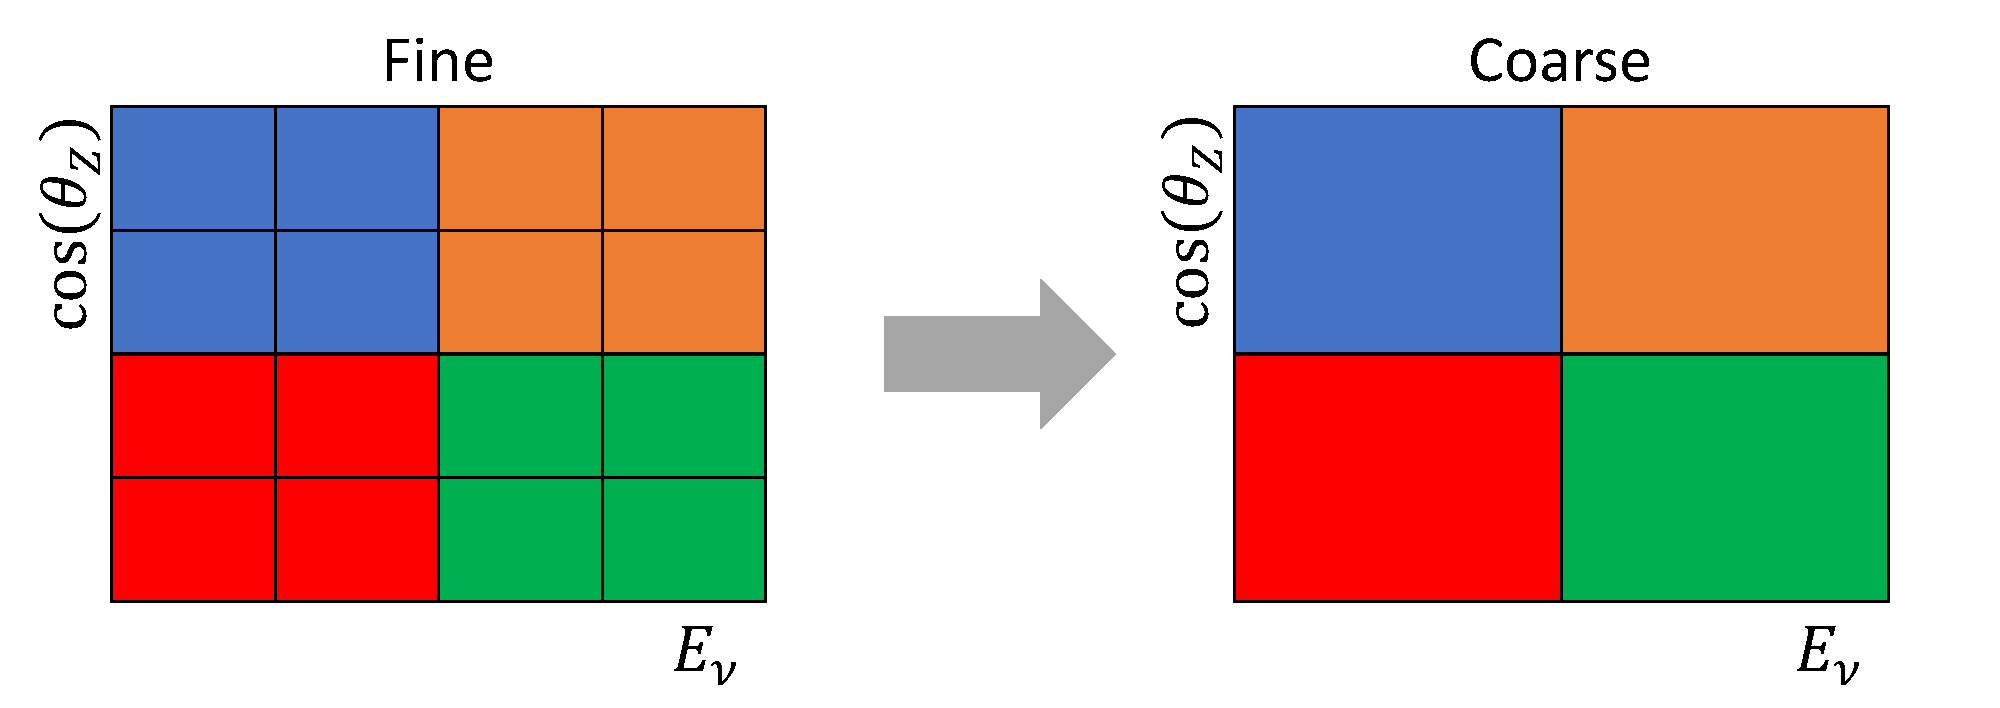
\includegraphics[width=\textwidth, trim={0mm 0mm 0mm 0mm}, clip,page=1]{Figures/Oscillation/SubSamplingExample.pdf}
  \end{subfigure}
  \caption{Illustration of the averaging procedure for \quickmath{N=2}. The oscillation probabilities calculated on the finer left binning are averaged to obtain the oscillation probabilities in the coarser right binning. These averaged oscillation probabilities with the coarser binning are then applied to each event during the fit.}
  \label{fig:Oscillation_SK_SubSamplingExample}
\end{figure}

The coarse binning is defined with \quickmath{67 \times 52} bins in true neutrino energy \quickmath{\times} cosine zenith. It is picked to be identical to that provided in \cite{t2k_tn_425}. In general, the binning is logarithmically spaced in neutrino energy but has some hand-picked bin edges around the matter resonance to smoothly increased the bin density. This is to avoid smearing this region which can be well sampled by the Monte Carlo. The cosine zenith binning is approximately linearly spaced across the allowable range but the values of layer transitions are hit precisely: \quickmath{-0.8376} (core-mantle) and \quickmath{-0.4464} (mantle/transition zone). Bins are spread further apart for downgoing events as this is a region unaffected by the fast oscillation wavelengths and reduces the total number of calculations required to perform the calculation.

The choice of \quickmath{N} is justified based on two studies. Firstly, the variation of event rates of each sample is studied as a function of \quickmath{N}. For a given set of oscillation parameters thrown from the PDG prior constraints (detailed in \autoref{tab:Theory_PDGConstraints}), the oscillation probabilities are calculated using a given value of \quickmath{N}. Each sample is re-weighted and the event rate is stored. The value of \quickmath{N} is scanned from \quickmath{1}, which corresponds to no averaging, to \quickmath{19}, which corresponds to the largest computationally viable subdivision binning. The event rate of each sample at large \quickmath{N} is expected to converge to a stationary value due to the fine binning fully sampling the small-scale structure. \autoref{fig:Oscillation_SK_EventRateVariable} illustrates this behaviour for the \texttt{SubGeV\_elike\_0dcy} sample for \quickmath{9} different throws of the oscillation parameters.

\begin{figure}[h]
  \begin{subfigure}[t]{\textwidth}
    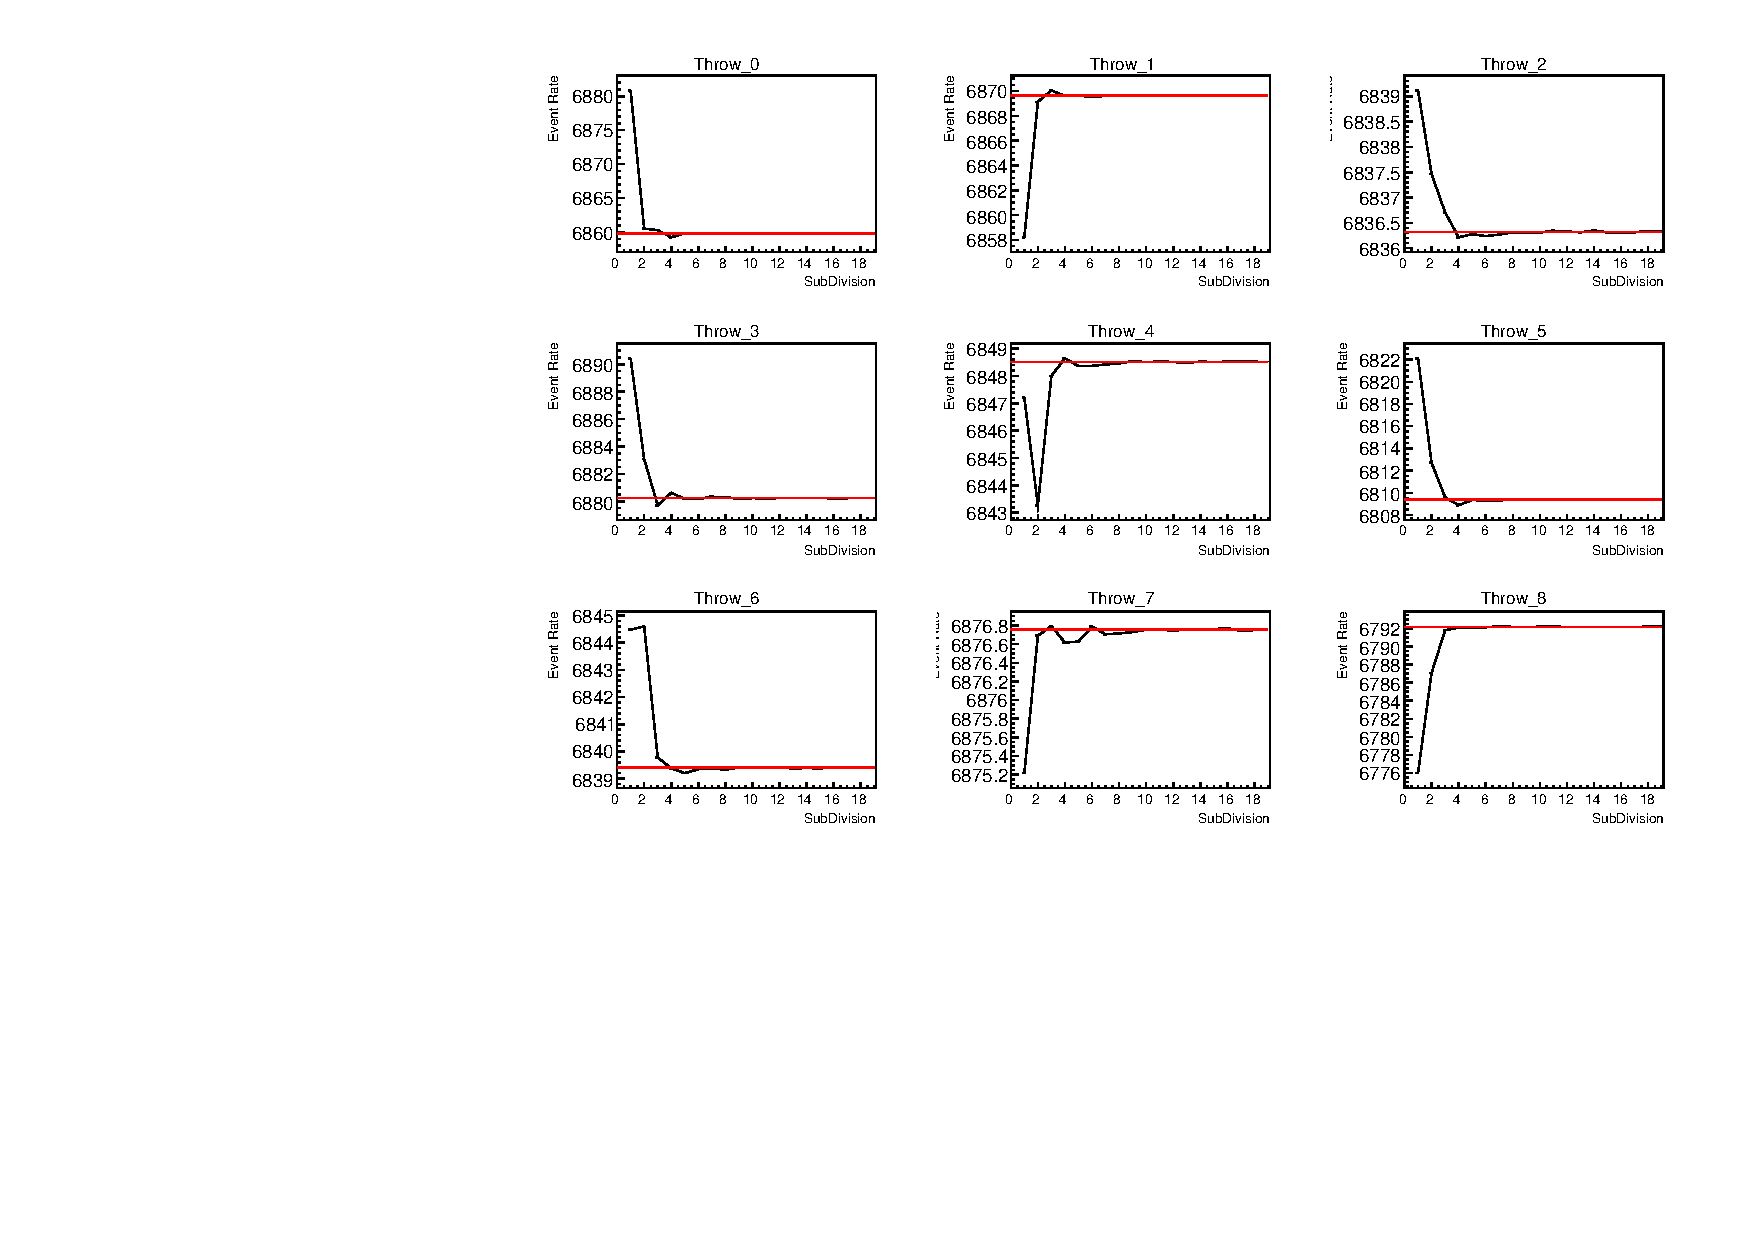
\includegraphics[width=\textwidth, trim={0mm 0mm 0mm 0mm}, clip,page=1]{Figures/Oscillation/EventRate_VariableGraphs.pdf}
  \end{subfigure}
  \caption{Event rate of the \texttt{SubGeV\_elike\_0dcy} sample as a function of the number of sub-divisions per coarse bin. Each subplot represents the event rate of the sample at a different oscillation parameter set thrown from the PDG priors detailed in \autoref{tab:Theory_PDGConstraints}. The red line in each subplot represents the mean of the event rate over the different values of sub-divisions for that particular oscillation parameter throw.}
  \label{fig:Oscillation_SK_EventRateVariable}
\end{figure}

Denoting the event rate for one sample for a given throw \quickmath{t} at each \quickmath{N} by \quickmath{\lambda_t^{N}}, the average over all considered \quickmath{N} values (\quickmath{\overline \lambda_t = \frac{1}{24} \sum_{N=1}^{24} \lambda_t^{N}}) is computed. The variance in the event rate at each \quickmath{N} is then calculated as

\begin{equation}
  \mathrm{Var}\Big[\lambda^{N}\Big] = \tfrac{1}{N_\mathrm{throws}} \sum_{t=1}^{N_\mathrm{throws}} \left(\lambda_t^{N} - \overline \lambda_t\right)^2 - \left[\tfrac{1}{N_\mathrm{throws}} \sum_{t=1}^{N_\mathrm{throws}} \left(\lambda_t^{N} - \overline \lambda_t\right)\right]^2 .
  \label{eq:Oscillation_SK_Variance}
\end{equation}

In practice, the following procedure is undertaken. For a particular throw, the difference between the event rate at a particular choice of \quickmath{N} and the mean of the distribution is calculated. This is illustrated in \autoref{fig:Oscillation_SK_ExampleCalculation}. This value is then calculated for all the \quickmath{2000} throws, generating a distribution of \quickmath{\lambda_t^{N} - \overline \lambda_t}. This is repeated for each of the values of \quickmath{N} considered within this study. The distributions of this value, for \quickmath{N = \{1,5\}}, are given in \autoref{fig:Oscillation_SK_DifferenceDistribution}. As expected, the distribution gets narrower and tends towards zero for the higher values of \quickmath{N}. 

\begin{figure}[h]                                                                                                                                                                                          
  \begin{subfigure}[t]{\textwidth}
    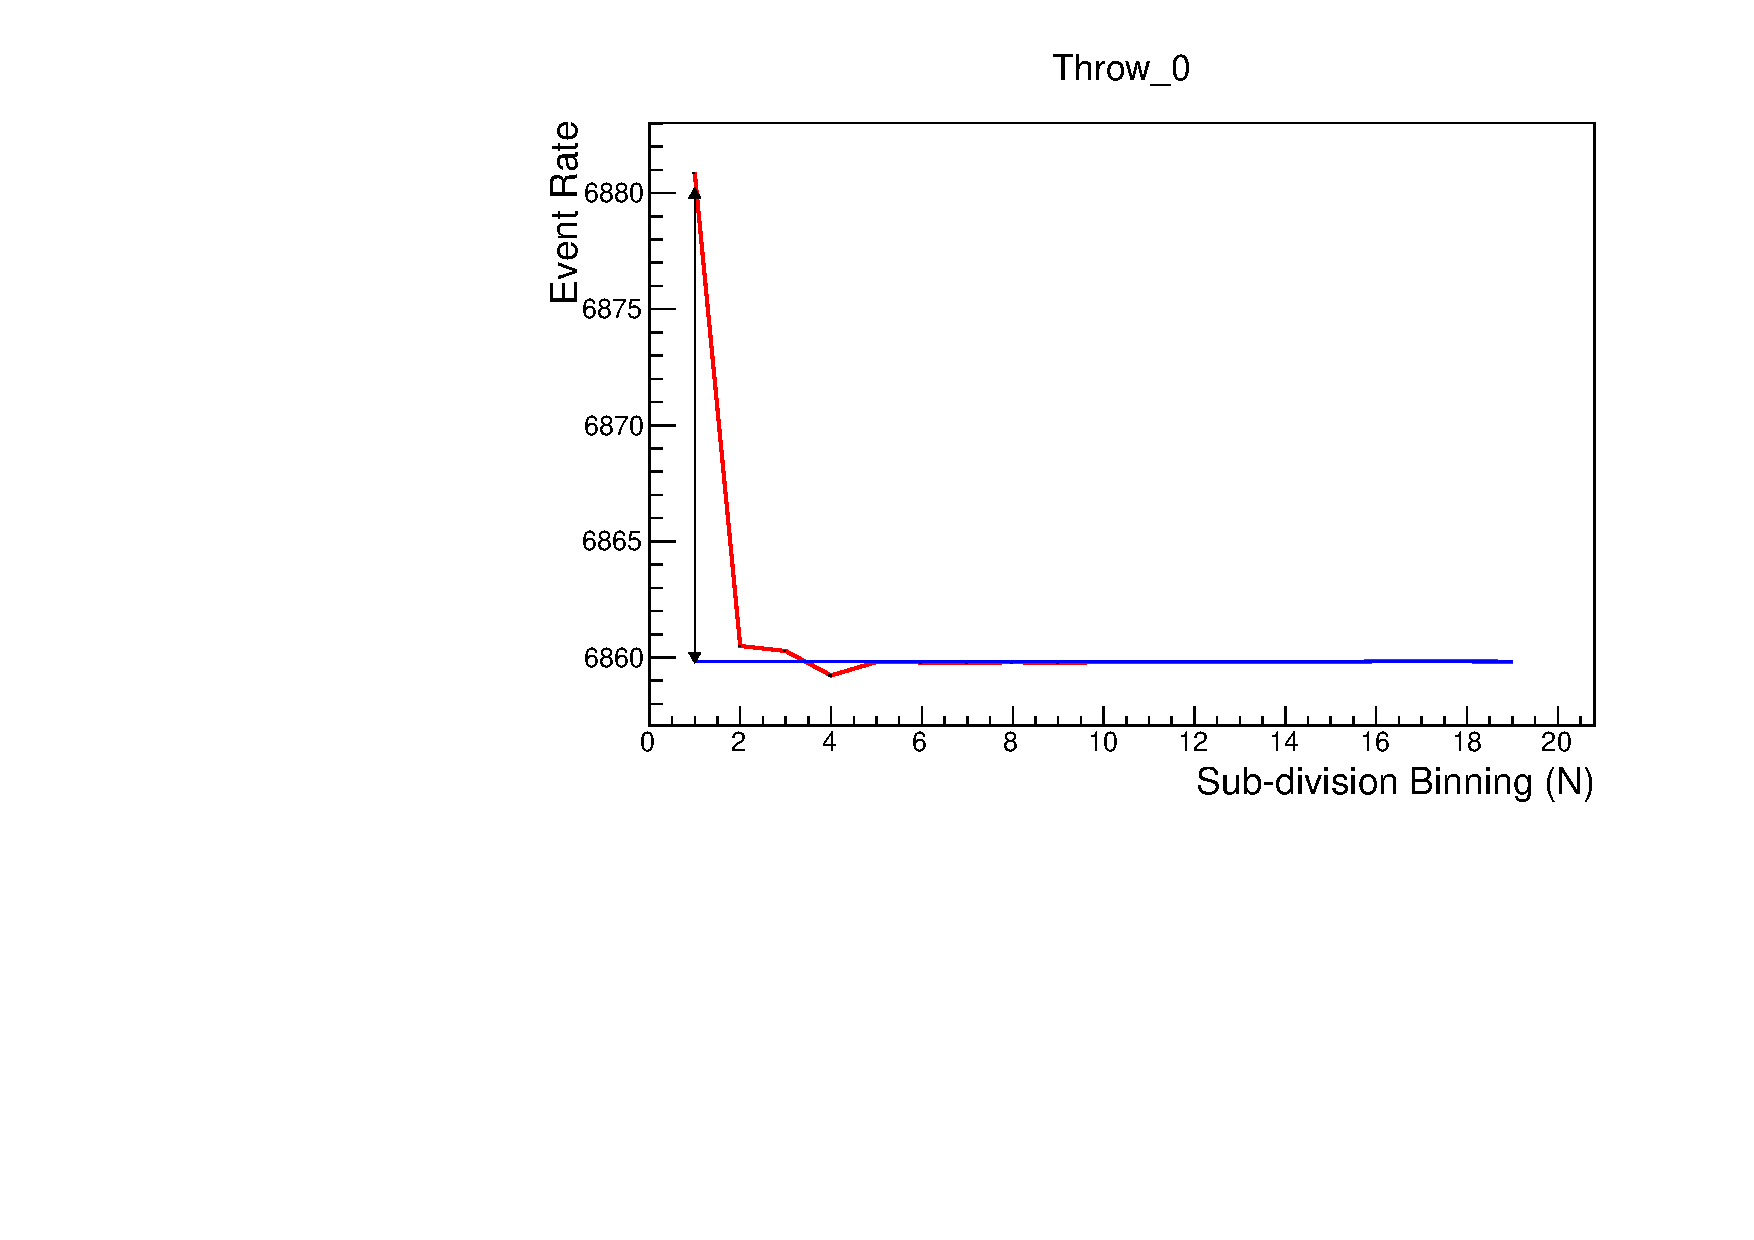
\includegraphics[width=\textwidth, trim={0mm 0mm 0mm 0mm}, clip,page=1]{Figures/Oscillation/ExampleCalculation.pdf}
  \end{subfigure}
  \caption{Event rate of the \texttt{SubGeV\_elike\_0dcy} sample, for a particular oscillation parameter throw, as a function of the number of sub-divisions, \quickmath{N}, per coarse bin. The difference between the mean event rate (red), \quickmath{\bar{\lambda}}, and the event rate at \quickmath{N=1}, \quickmath{\lambda^{N=1}} is defined as \quickmath{\lambda^{N} - \bar{\lambda}} and illustrated by the blue arrow.}
  \label{fig:Oscillation_SK_ExampleCalculation}
\end{figure}

\begin{figure}[h]                                                                                                                                                                                          
  \begin{subfigure}[t]{\textwidth}
    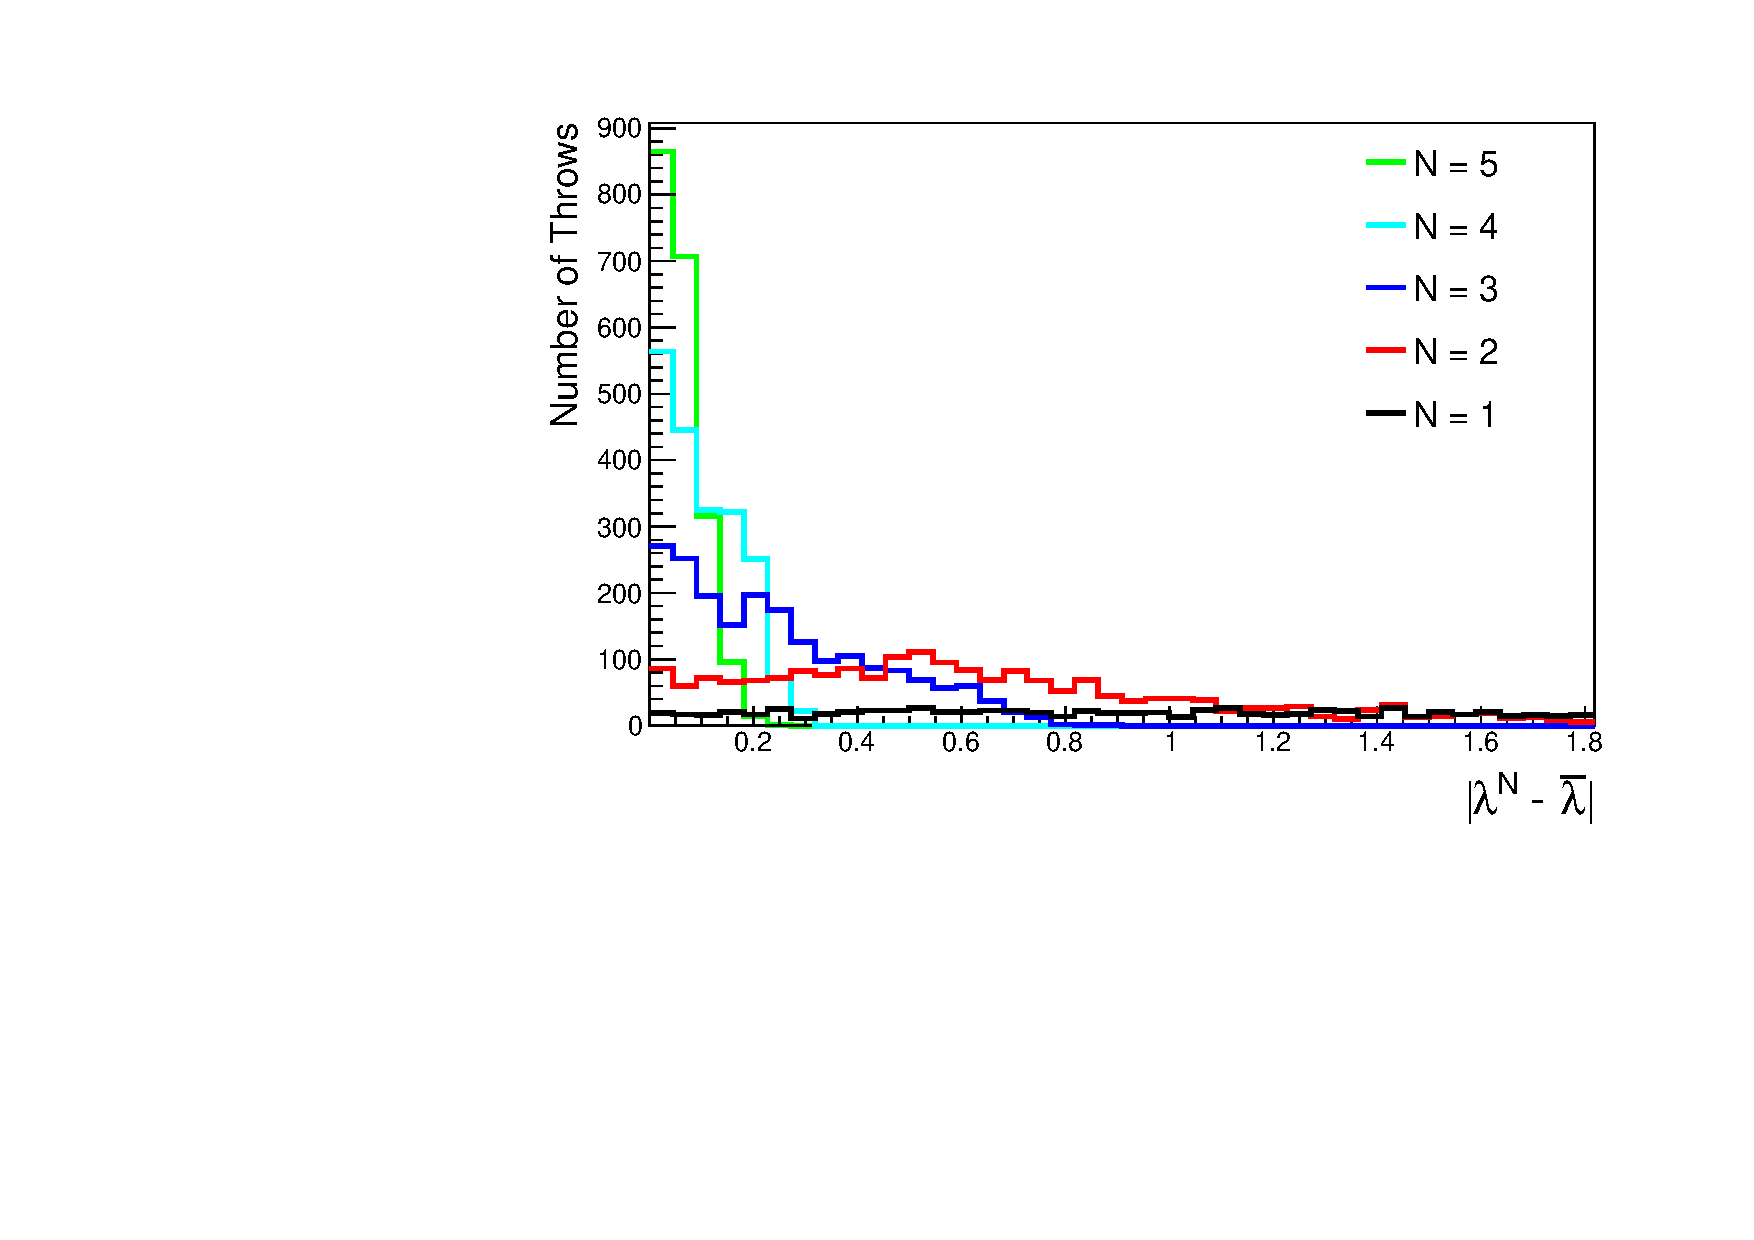
\includegraphics[width=\textwidth, trim={0mm 0mm 0mm 0mm}, clip,page=1]{Figures/Oscillation/DifferenceInEventRateToMean.pdf}
  \end{subfigure}
  \caption{The distribution of \quickmath{\lambda^{N} - \bar{\lambda}} for various values of \quickmath{N}. As expected, the distribution gets narrower for larger values of \quickmath{N}.}
  \label{fig:Oscillation_SK_DifferenceDistribution}
\end{figure}

The aim of the study is to find the lowest value of \quickmath{N} such that this variance is below \quickmath{0.001}. This utilises the width of the distributions given in \autoref{fig:Oscillation_SK_DifferenceDistribution}. This is the typical threshold used by T2K fitters to validate systematic implementation so has been set as the same criteria. The results of this study for each atmospheric sample used within this thesis are illustrated in \autoref{fig:Oscillation_SK_EventRateVariance} for \quickmath{2000} throws of the oscillation parameters. As can be seen, the variance is below the threshold at \quickmath{N = 10}, and is driven primarily by the \texttt{SubGeV\_mulike\_1dcy} and \texttt{SubGeV\_elike\_0dcy} samples.

%\begin{figure}[h]
\begin{sidewaysfigure}
  \begin{subfigure}[t]{\textwidth}
    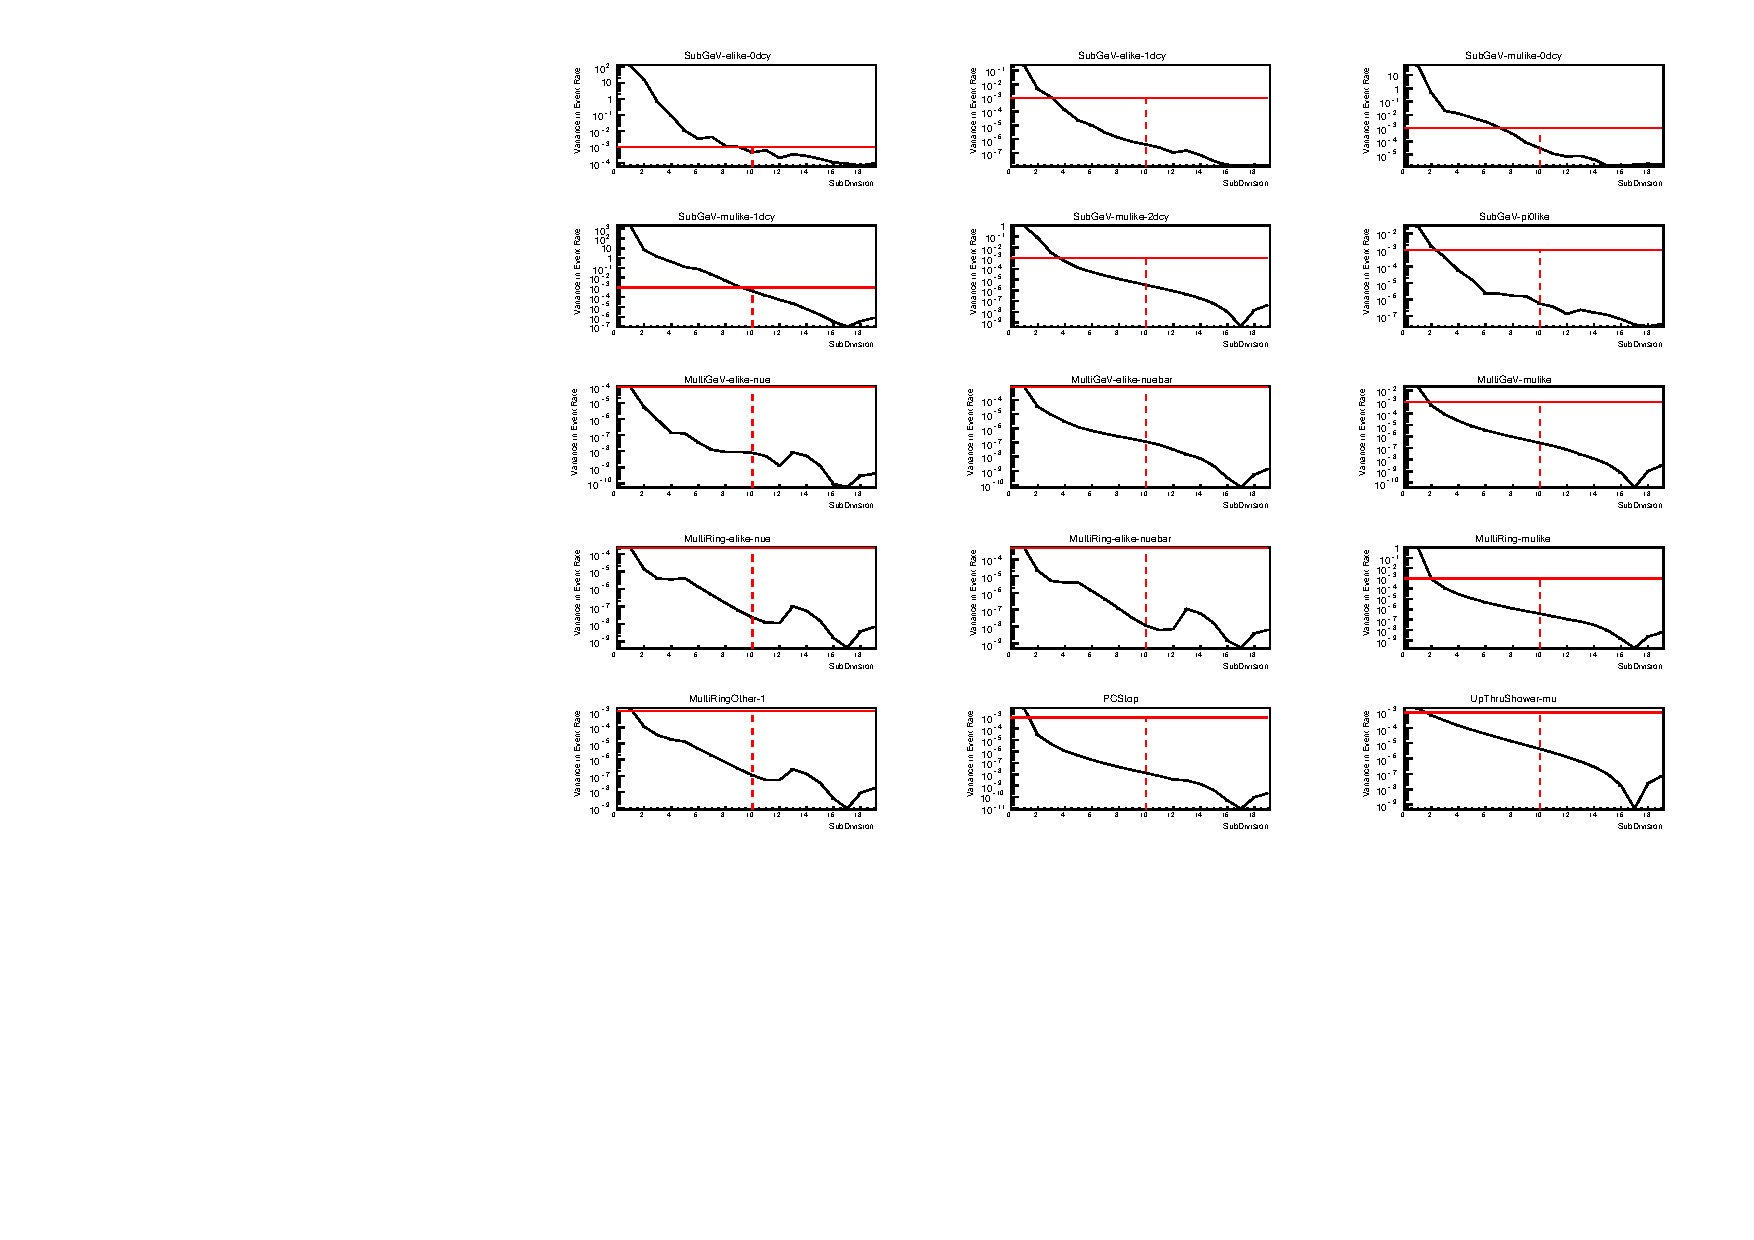
\includegraphics[width=\textwidth, trim={0mm 0mm 0mm 0mm}, clip,page=1]{Figures/Oscillation/EventRate_VarianceGraphs.pdf}
  \end{subfigure}
  \caption{Variance of event rate for each atmospheric sample as a function of the number of sub-divisions per coarse bin. The solid red line indicates the \quickmath{0.1\%} threshold and the dashed red line indicates the variance at a sub-division \quickmath{N = 10}.}
  \label{fig:Oscillation_SK_EventRateVariance}
\end{sidewaysfigure}
  %\end{figure}
  

The second study to determine the value of \quickmath{N} is as follows. The likelihood for each sample is computed against an Asimov data set created with Asimov A oscillation parameters (\autoref{tab:Theory_ParameterSets}). Following \autoref{eq:Oscillation_SK_Variance}, the variance of the log-likelihood over all considered \quickmath{N} is computed. The results are shown in \autoref{fig:Oscillation_SK_LLHVariance}. 

%\begin{figure}[h]
\begin{sidewaysfigure}
  \begin{subfigure}[t]{\textwidth}
    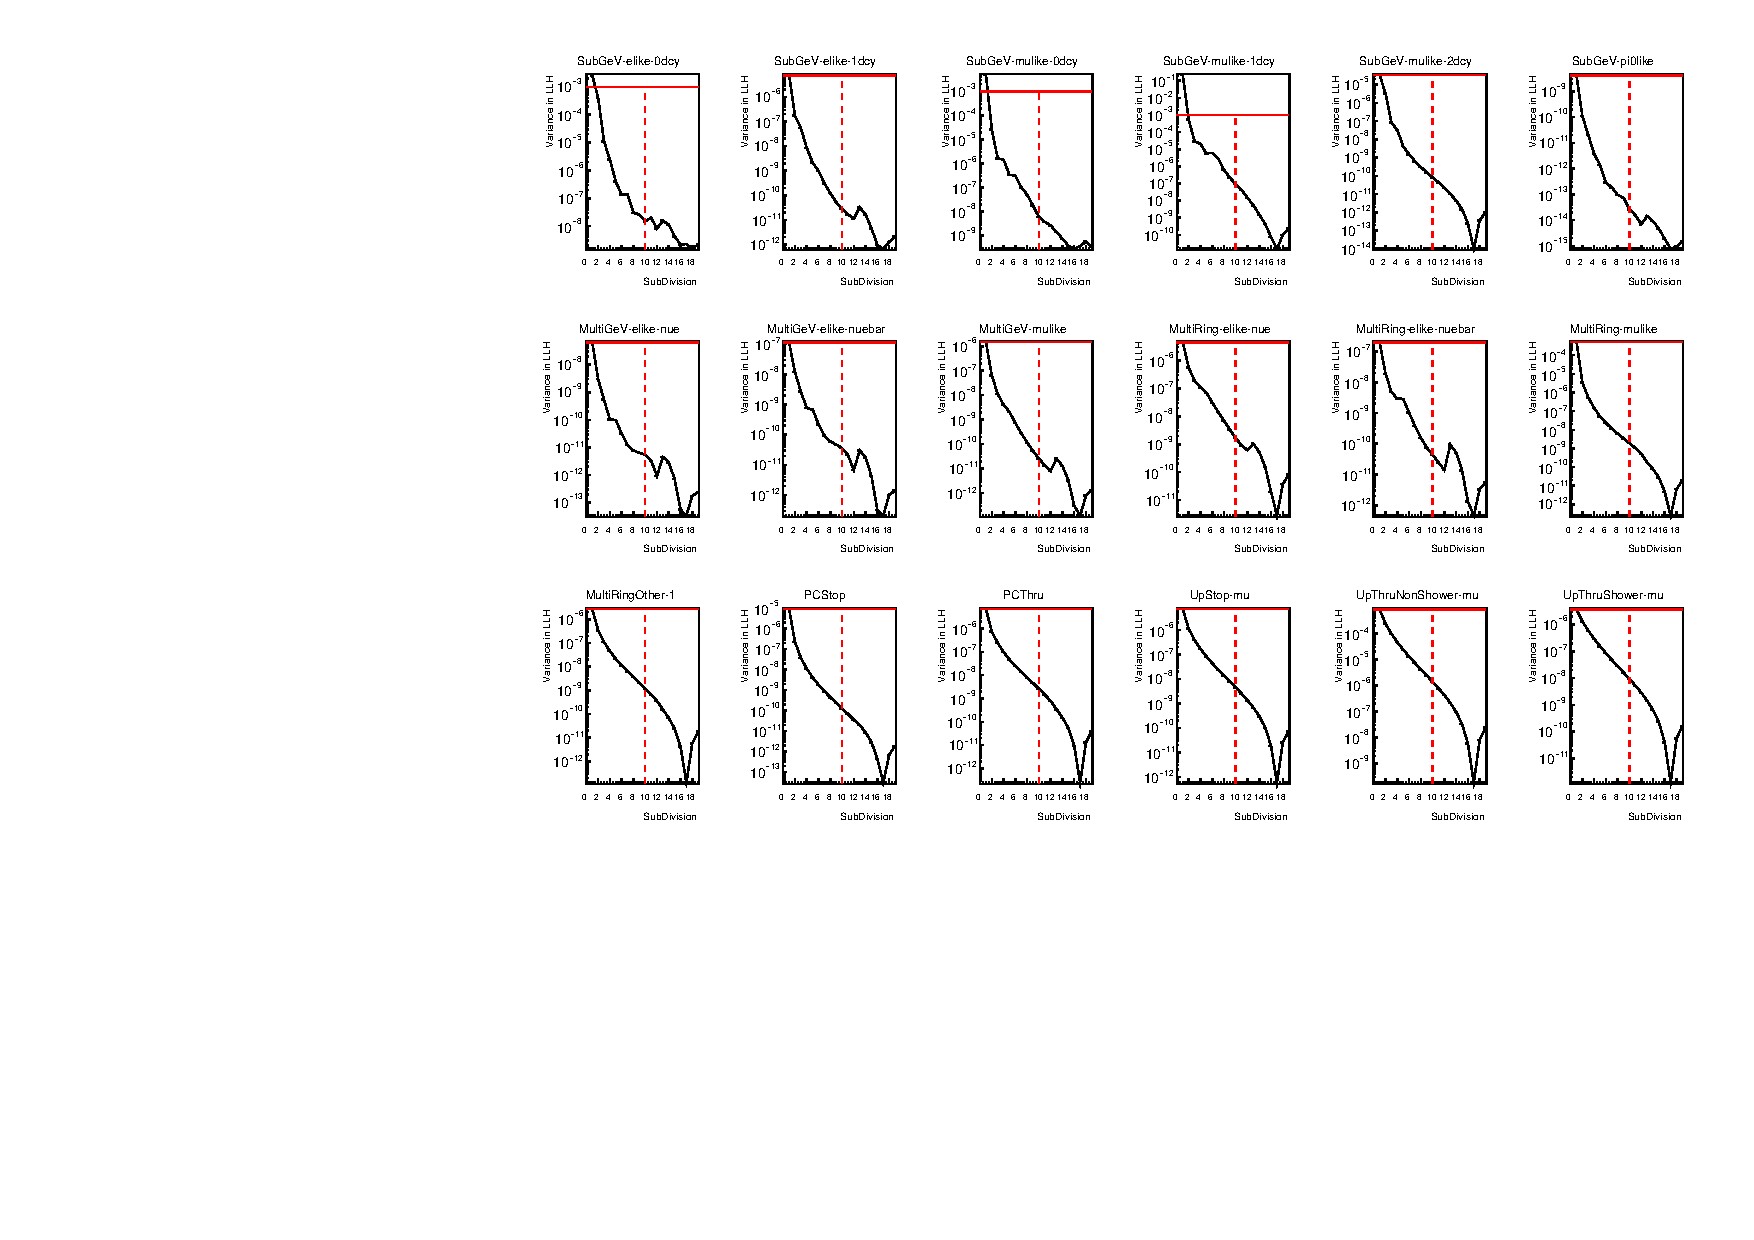
\includegraphics[width=\textwidth, trim={0mm 0mm 0mm 0mm}, clip,page=1]{Figures/Oscillation/Likelihood_VarianceGraphs.pdf}
  \end{subfigure}
  \caption{Variance of sample likelihood, when compared to `Asimov data' set at Asimov A, for each atmospheric sample as a function of the number of sub-divisions per coarse bin. The solid red line indicates the \quickmath{0.1\%} threshold and the dashed red line is a graphical indication of the variance at a sub-division \quickmath{N = 10}.}
  \label{fig:Oscillation_SK_LLHVariance}
\end{sidewaysfigure}
%\end{figure}

A choice of \quickmath{N=10} sub-divisions per coarse bin has a variance in both event rate and log-likelihood residuals less than the required threshold of \quickmath{0.001}. The largest value of the likelihood variance is of order \quickmath{10^{-7}}, corresponding to an error on the log-likelihood of about \quickmath{3\times 10^{-4}} which is small enough to be negligible for the oscillation analysis.

\autoref{fig:Oscillation_SK_SmearingImplementation} illustrates the effect of the smearing using \quickmath{N = 10}. The fast oscillations in the sub-GeV upgoing region have been replaced with a normalisation effect whilst the large matter resonance structure remains.

\begin{figure}[h]
  \begin{subfigure}[t]{\textwidth}
    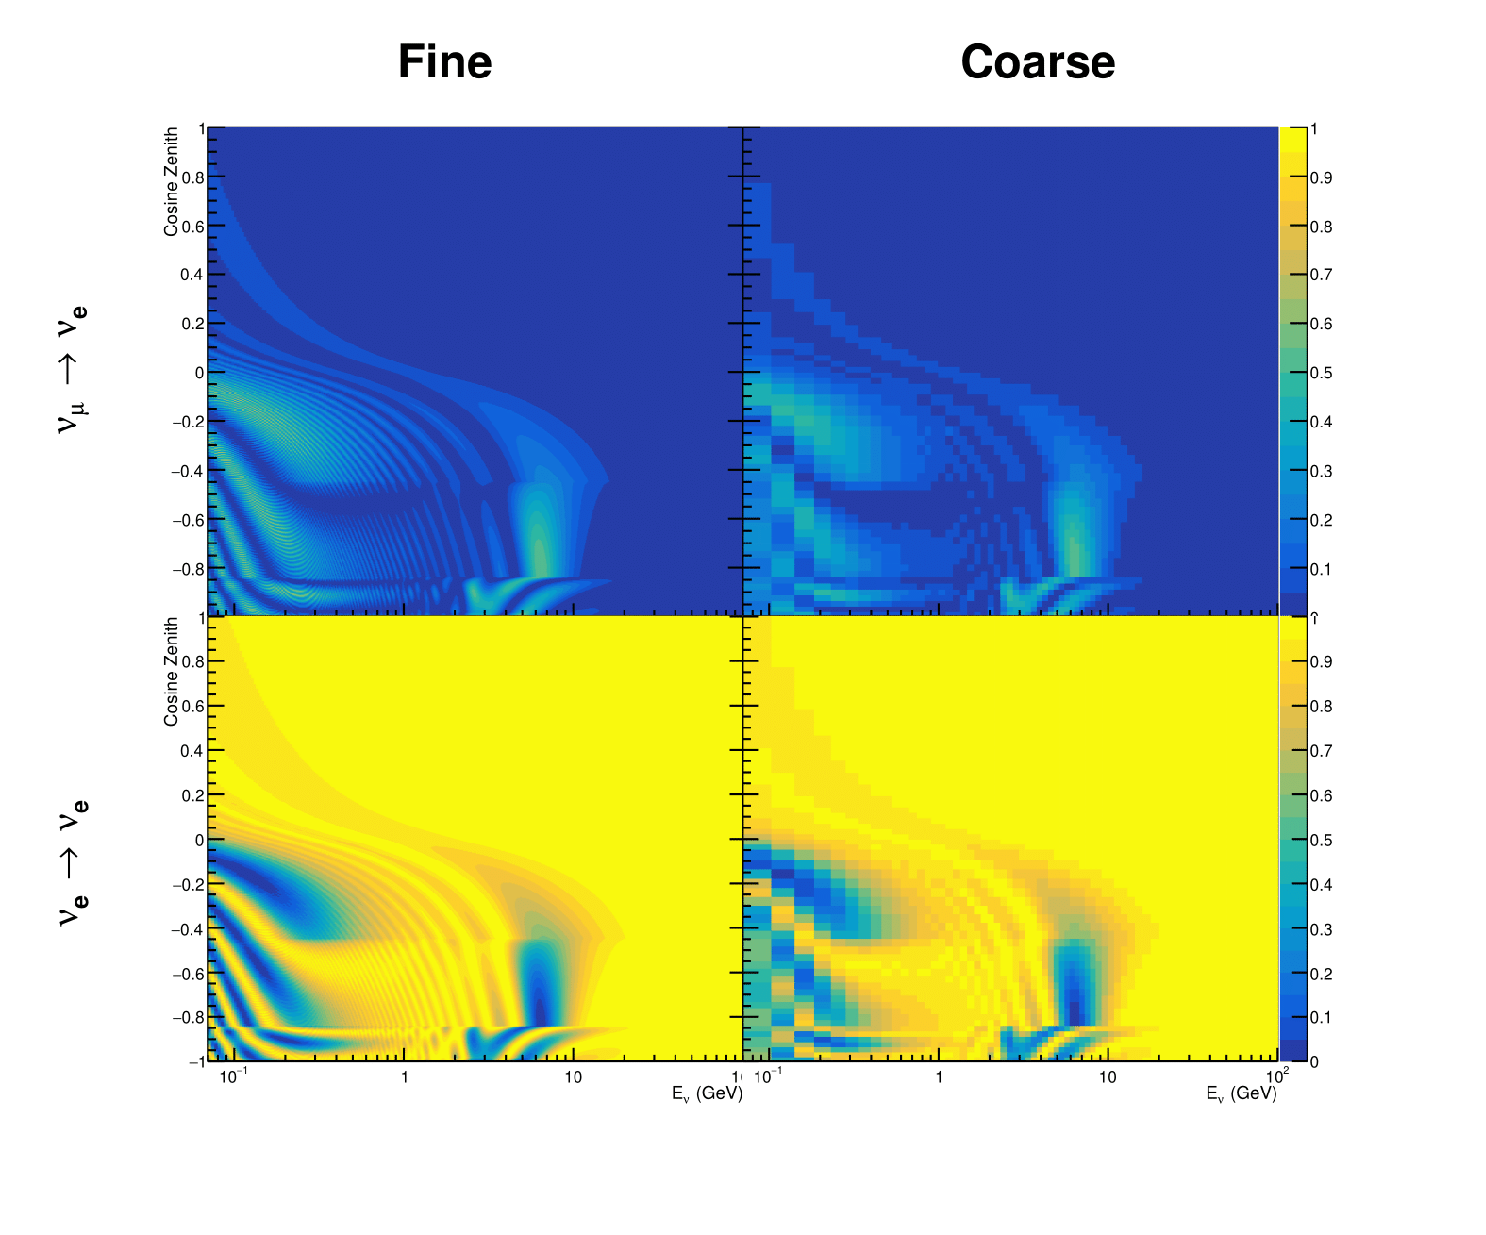
\includegraphics[width=\textwidth, trim={0mm 0mm 0mm 0mm}, clip,page=1]{Figures/Oscillation/SmearingImplementation.pdf}
  \end{subfigure}
  \caption{The oscillation probability, \quickmath{P(\nu_{\mu} \rightarrow \nu_{e})} (top row) and \quickmath{P(\nu_{e} \rightarrow \nu_{e})} (bottom row), given as a function of neutrino energy and zenith angle. The left column gives the ``fine'' binning used to calculate the oscillation probabilities and the right column illustrates the ``coarse'' binning used to reweight the Monte Carlo events. The fine binning choice is given with \quickmath{N = 10}, which was determined to be below the threshold from \autoref{fig:Oscillation_SK_EventRateVariance} and \autoref{fig:Oscillation_SK_LLHVariance}.}
  \label{fig:Oscillation_SK_SmearingImplementation}
\end{figure}

\section{Calculation Engine}
\label{sec:Oscillation_CalculationEngine}

As previously discussed in \autoref{sec:Oscillation_FastOscillations}, the calculation of oscillation probabilities is performed at run-time. Consequently, the time per calculation is crucial for fit performance. The initial fitting framework used for this analysis was developed with \texttt{ProbGPU} \cite{probgpu}. This is a GPU-only implementation of the \text{prob3} engine \cite{Prob3}. It is primarily designed for neutrino propagation in a beam experiment (single layer of constant density) with the atmospheric propagation code not being used prior to the analysis in this thesis.

Another engine, \texttt{CUDAProb3} \cite{cudaprob3}, has been interfaced with the fitting framework used in this analysis. This interfacing was done by the author of this thesis. It has been specifically optimised for atmospheric neutrino oscillation calculation so does not contain the code to replace the beam oscillation calculation. The engine utilises object-orientated techniques as compared to the functional implementation of \texttt{ProbGPU}. This allows the energy and cosine zenith arrays to be kept on GPU memory, rather than having to load these arrays onto GPU memory for each calculation. Reducing the memory transfer between CPU and GPU significantly reduces the time required for calculation. This can be seen in \autoref{fig:Oscillation_CalculationTime}, where the GPU implementation of \texttt{CUDAProb3} is approximately three times faster than the \texttt{ProbGPU} engine. 

\begin{figure}[h]
  \begin{subfigure}[t]{0.8\textwidth}
    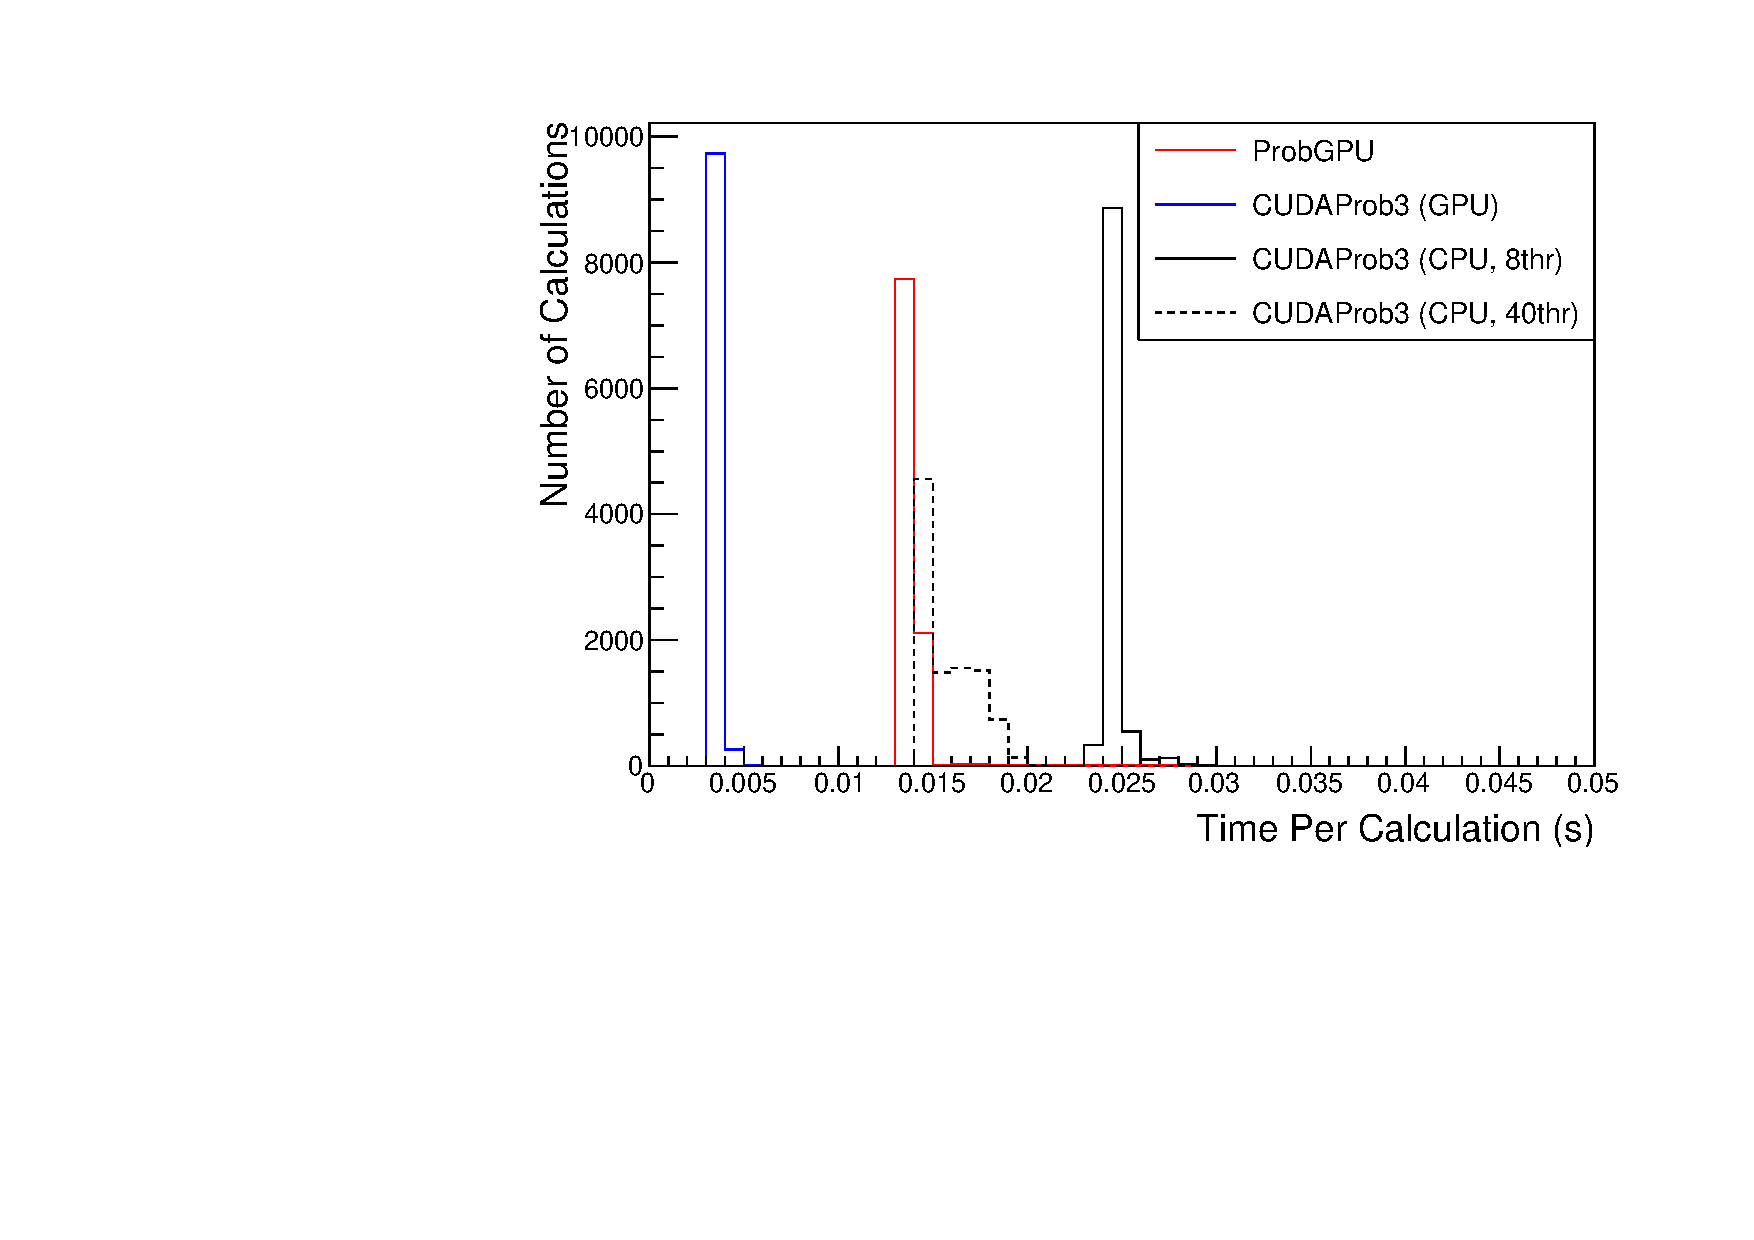
\includegraphics[width=\textwidth, trim={0mm 0mm 0mm 0mm}, clip,page=1]{Figures/Oscillation/CalculationTime.pdf}
  \end{subfigure}
  \caption{The calculation time taken to both calculate the oscillation probabilities and fill the ``coarse'' oscillograms, following the technique given in \autoref{sec:Oscillation_FastOscillations},  for the \texttt{CUDAProb3} and \texttt{ProbGPU} (Red) calculation engines. \texttt{CUDAProb3} has both a GPU (Blue) and CPU (Black) implementation, where the CPU implementation is multi-threaded. Therefore, 8-threads (solid) and 40-threads (dashed) configurations have been tested. \texttt{Prob3}, which is a CPU single-thread implementation has a mean step time of \quickmath{1.142\text{s}}.}
  \label{fig:Oscillation_CalculationTime}
\end{figure}

Another significant advantage of \texttt{CUDAProb3} is that it contains a CPU multithreaded implementation which is not possible with the \texttt{ProbGPU} or \texttt{prob3} engines. This eliminates the requirement for GPU resources when submitting jobs to batch systems. As illustrated in \autoref{fig:Oscillation_CalculationTime}, the calculation speed depends on the number of available threads. Using \quickmath{8} threads (which is typical of the batch systems being used) is approximately twice as slow as the \texttt{ProbGPU} engine implementation, but would allow the fitting framework to be run on many more resources. This fact is utilised for any SK-only fits but GPU resources are required for any fits which include beam samples due to the \texttt{ProbGPU} requirement. Based on the benefits shown by the implementation in this section, efforts are being placed into including linear propagation for beam neutrino propagation into the engine \cite{Liban}.

\section{Matter Density Profile}
\label{sec:Oscillation_MatterDensity}


For an experiment observing neutrinos propagating through the Earth, a model of the Earth's density profile is required. The model used within this analysis is based on the Preliminary Reference Earth Model (PREM) \cite{Dziewonski1981-sp}, as illustrated in \autoref{fig:Oscillation_SK_PREMModelApproximation}. \autoref{tab:NeutrinoOscillationPhysics_PREMModel} documents the density and radii of the layers used within the constant density approximation used by the SK-only analysis \cite{thesis_roger}. The density measurements provided in the PREM model are provided in terms of mass density, whereas neutrino oscillations are sensitive to the electron number density. This value can be computed as the product of the chemical composition, or the \quickmath{Z/A} value, and the mass density of each layer. Currently, the only way to measure the chemical composition value for layers close to the Earth's core is through neutrino oscillations. The chemical composition of the upper layers of the Earth's Mantle and the Transition zone is well known due to it being predominantly pyrolite which has a chemical composition value of \quickmath{0.496} \cite{Bourret_2017}. The chemical composition dial for the core layers is set to a value of \quickmath{0.468}, as calculated in \cite{Rott2015}. As this value is less well known, it is assigned a Gaussian error with a standard deviation equivalent to the difference in chemical composition in core and mantle layers. \autoref{fig:Oscillation_SK_ChemicalComposition} illustrates the effect of moving from the \quickmath{Z/A = 0.5} method which is used in the official SK-only analysis to these more precise values.

%For an experiment observing neutrinos propagating through the Earth, a model of the Earth's density profile is required. The model used within this analysis is based on the Preliminary Reference Earth Model (PREM) \cite{Dziewonski1981-sp}, as illustrated in \autoref{fig:Oscillation_SK_PREMModelApproximation}. \autoref{tab:NeutrinoOscillationPhysics_PREMModel} documents the density and radii of the layers used within the constant density approximaton ued b the SK-only analysis \cite{thesis_roger}. The density measurements provided in the PREM model are provided in terms of mass density, whereas neutrino oscillations are sensitive to the electron number density. This value can be computed as the product of the chemical composition, or the \quickmath{Z/A} value, and the mass density of each layer. Currently, the only way to measure the chemical composition value for layers close to the Earth's core is through neutrino oscillations. The chemical composition of the upper layers of the Earth's Mantle and the Transition zone is well known due to it being predominantly pyrolite which has a chemical composition value of \quickmath{0.496} \cite{Bourret_2017}. The chemical composition dial for the core layers is set to a value of \quickmath{0.468}, as calculated in \cite{Rott2015}. As this value is less well known, it is assigned a Gaussian error with a standard deviation equivalent to the difference in chemical composition in core and mantle layers. \autoref{fig:Oscillation_SK_ChemicalComposition} illustrates the effect of moving from the \quickmath{Z/A = 0.5} method which is used in the official SK-only analysis \cite{thesis_roger} to these more precise values.

\begin{figure}[h]
  \begin{subfigure}[t]{\textwidth}
    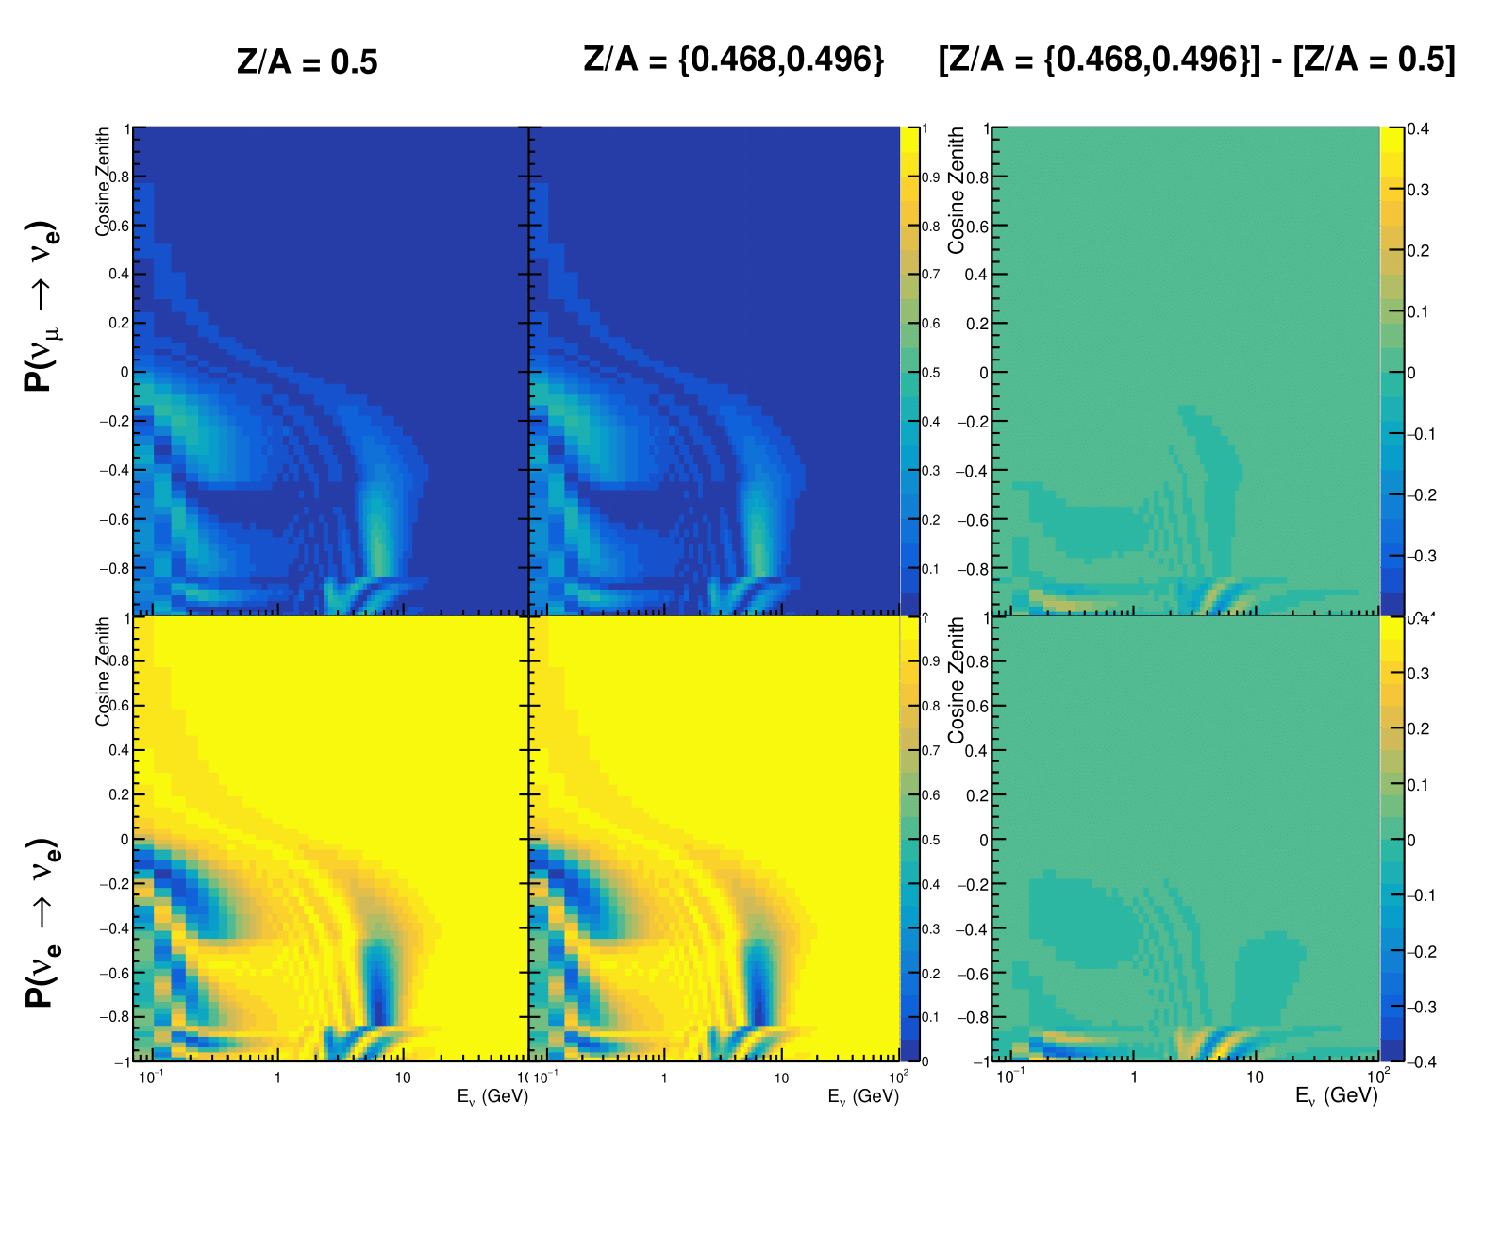
\includegraphics[width=\textwidth, trim={0mm 0mm 0mm 0mm}, clip,page=1]{Figures/Oscillation/ChemicalComposition.pdf}
  \end{subfigure}
  \caption{The oscillation probability, \quickmath{P(\nu_{\mu} \rightarrow \nu_{e})} (top row) and \quickmath{P(\nu_{e} \rightarrow \nu_{e})} (bottom row), given as a function of neutrino energy and zenith angle. The left column gives probabilities where the constant \quickmath{Z/A = 0.5} approximation which is used in the official SK-only analysis. The middle column gives the probabilities where \quickmath{Z/A = [0.468,0.498]} values are used, as given in \autoref{tab:NeutrinoOscillationPhysics_PREMModel}. The right column illustrates the difference in oscillation probability between the two different techniques.}
  \label{fig:Oscillation_SK_ChemicalComposition}
\end{figure}

The beam oscillation probability in this thesis uses a baseline of \quickmath{295 \text{km}}, density \quickmath{2.6 \text{g/cm}^{3}}, and chemical composition \quickmath{0.5} as is done by the official T2K-only analysis \cite{Hagiwara2011}. 

%Whilst the propagator requires a fixed density layer model of the Earth, the density only has to be fixed for a specific \quickmath{E_{\nu} \times \cos(\theta_{Z})} bin in a given layer. As the density is a function of radius, which is a function of the direction in which a neutrino propagates, a better approximation of the PREM model can be made if a \quickmath{\cos(\theta_{Z})}-specific density is calculated. To achieve this, the average density, \quickmath{\left< \rho \right>_{i}}, in the \quickmath{i^{th}} layer, is calculated as the density, \quickmath{\rho(t)}, integrated over the track a given \quickmath{\cos(\theta_{Z})},

For a neutrino with given \quickmath{E_{\nu}}, \quickmath{\cos(\theta_{Z})}, the oscillation probability calculation engine must be passed a list of the matter regions that the neutrino traversed, with the path length and fixed density in each region. However, a neutrino passing through the earth experiences a range of radii, and thus a range of densities, in each region. In the SK-only analysis, the earth density model used is piecewise-constant, thereby ignoring this effect. For this thesis, the density values for the calculation engine are found by averaging the earth density along the neutrino's path in each layer,

\begin{equation}
  \left< \rho \right>_{i} = \frac{1}{t_{i+1}-t_{i}} \int^{t_{i}+1}_{t_{i}} \rho(t) dt,
\end{equation}

where \quickmath{t_{i}} are the intersection points between each layer and \quickmath{t} is the path length of the trajectory across the layer. This leads to an improved approximation. For this averaging, the simplification of the PREM model developed in \cite{EarthGrav} is used. The layers of the prem model are combined into four to reduce calculation time, with a quadratic fit to each section. This fit was not performed by the author of the thesis and is documented in \cite{t2k_tn_425}. The coefficients of the quadratic fit to each layer are given in \autoref{tab:NeutrinoOscillationPhysics_AveragePREMModel} with the final distribution illustrated in \autoref{fig:Oscillation_SK_PREMModelApproximationWithAveragePREMModel}. The quadratic approximation is clearly much closer to the PREM model as compared to the constant density approximation. 

%The oscillation probability calculation time is approximately linear in the number of layers invoked within the Earth model. Therefore a four-layer model is still utilized with the only difference to the official SK-only analysis being that the four-layer model used for each value of \quickmath{\cos(\theta_{Z})} is different. Following the method outlined in \cite{EarthGrav}, a four-layer piecewise quadratic polynomial is fit to the PREM model for the four layers defined in \autoref{tab:NeutrinoOscillationPhysics_PREMModel}. This fit was not performed by the author of the thesis and is documented in \cite{t2k_tn_425}. The coefficients of the quadratic fit to each layer are given in \autoref{tab:NeutrinoOscillationPhysics_AveragePREMModel} with the final distribution illustrated in \autoref{fig:Oscillation_SK_PREMModelApproximationWithAveragePREMModel}. The quadratic approximation is clearly much closer to the PREM model as compared to the constant density approximation. 

\begin{figure}[h]
  \begin{subfigure}[t]{0.8\textwidth}
    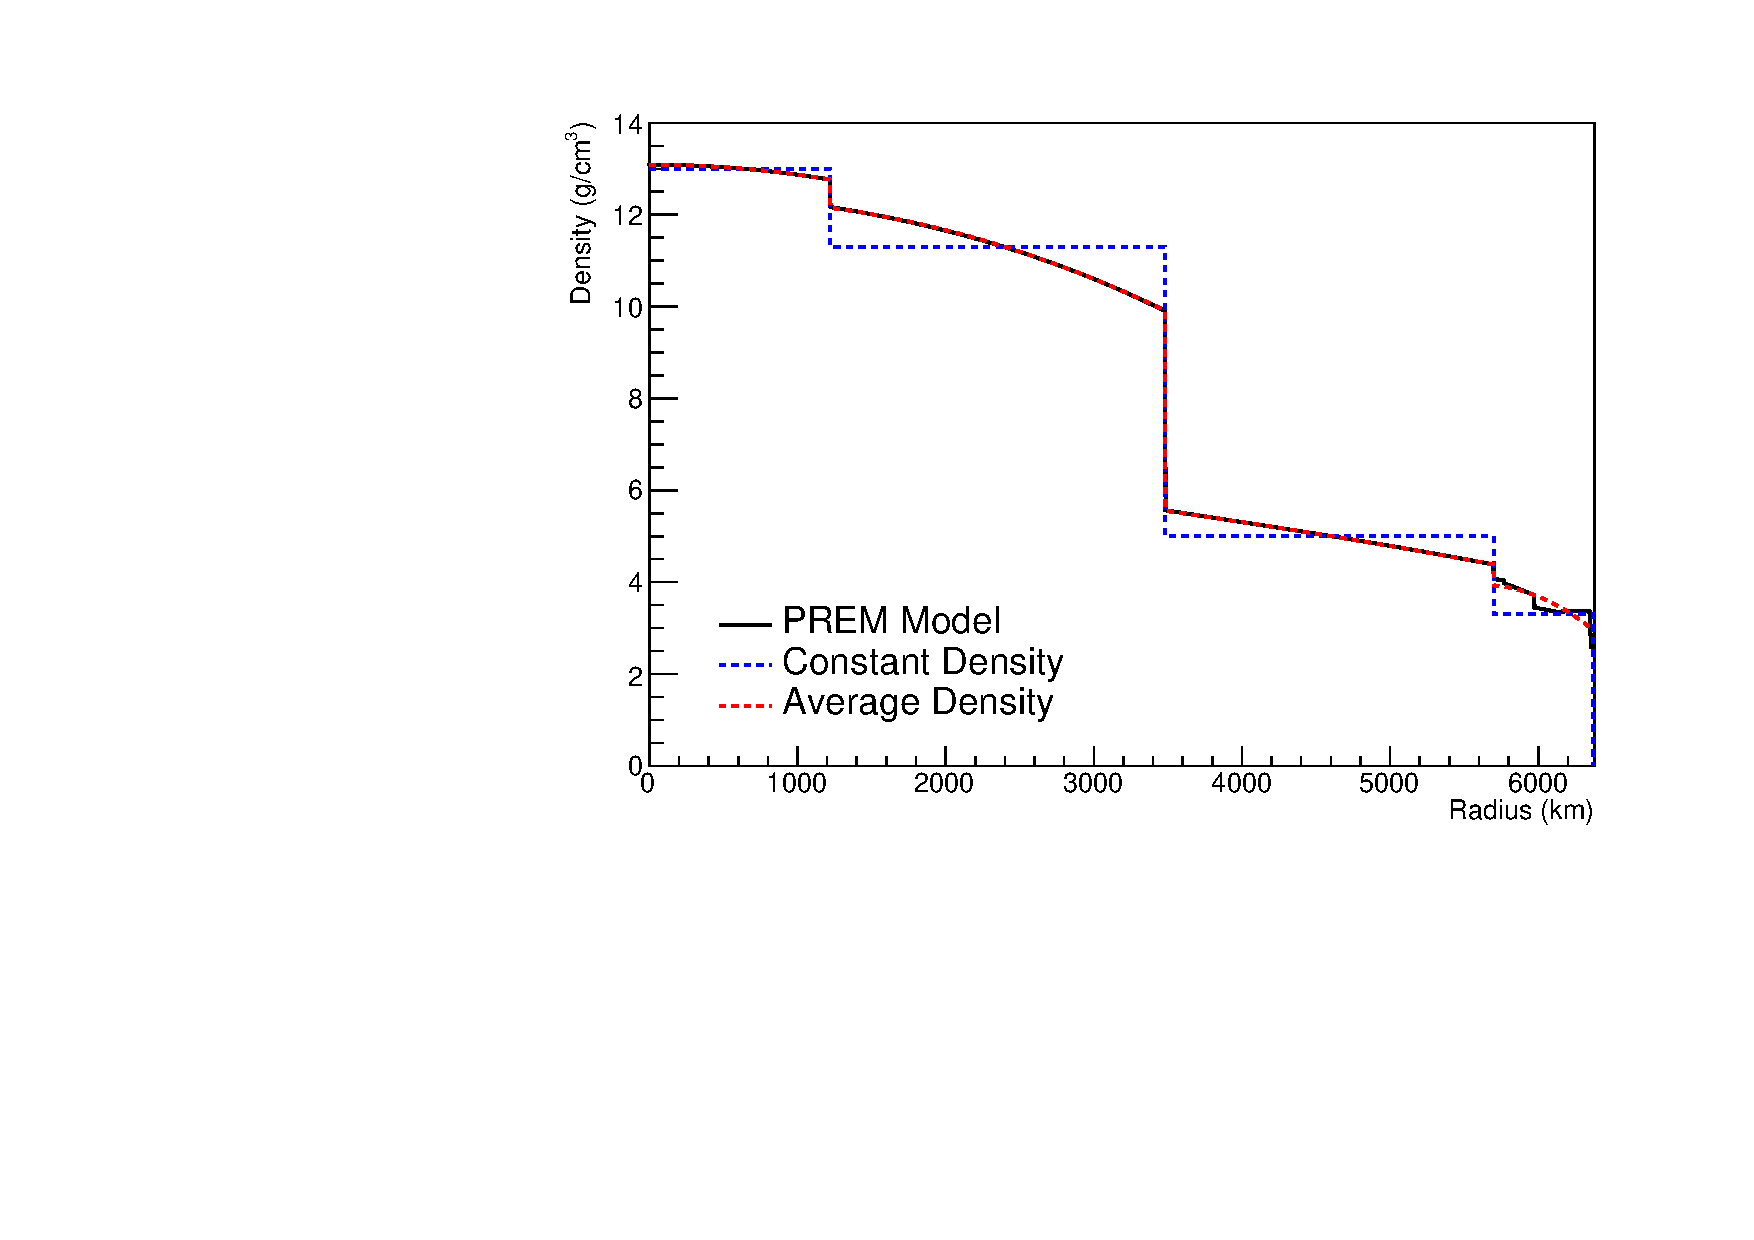
\includegraphics[width=\textwidth, trim={0mm 0mm 0mm 0mm}, clip,page=1]{Figures/Oscillation/DensityComparisonWithAveragePREM.pdf}
  \end{subfigure}
  \caption{The density of the Earth given as a function of the radius, as given by the PREM model (Black), the constant density four-layer approximation (Blue), as used in the official SK-only analysis, and the quadratic approximation of the PREM model (Red).}
  \label{fig:Oscillation_SK_PREMModelApproximationWithAveragePREMModel}
\end{figure}

\begin{table}[ht!]
    \centering
    \begin{tabular}{c|c|c}
      \hline
      Layer & Outer Radius [\quickmath{\text{km}}] & Density [\quickmath{\text{g/cm}^{3}}] \\
      \hline
      Inner Core & \quickmath{1220} & \quickmath{13.09 - 8.84 x^{2}} \\
      Outer Core & \quickmath{3480} & \quickmath{12.31 + 1.09 x - 10.02 x^{2}} \\
      Lower Mantle & \quickmath{5701} & \quickmath{6.78 - 1.56 x - 1.25 x^{2}} \\
      Transition Zone & \quickmath{6371} & \quickmath{-50.42 + 123.33 x - 69.95 x^{2}} \\
      \hline
    \end{tabular}
    \caption{The quadratic polynomial fits to the PREM model for four assumed layers of the PREM model. The fit to calculate the coefficients is given in \cite{t2k_tn_425}, where \quickmath{x = R/R_{Earth}}.}
    \label{tab:NeutrinoOscillationPhysics_AveragePREMModel}
\end{table}

The effect of using the quadratic density per \quickmath{\cos(\theta_{Z})} model is highlighted in \autoref{fig:Oscillation_SK_AverageDensityPREMModel}. The slight discontinuity in the oscillation probability around \quickmath{\cos(\theta_{Z}) \sim -0.45} in the fixed density model, which is due to the transition to mantle layer boundary, has been reduced. This is expected as the difference in the density across this boundary is significantly smaller in the quadratic density model as compared to the constant density model. Whilst the difference in density across the other layer transitions is reduced, there is still a significant difference. This means the discontinuities in the oscillation probabilities remain but are significantly reduced. However, as the quadratic density approximation matches the PREM model well in this region, these discontinuities are due to the Earth model rather than an artifact of the oscillation calculation.

\begin{figure}[h]
  \begin{subfigure}[t]{\textwidth}
    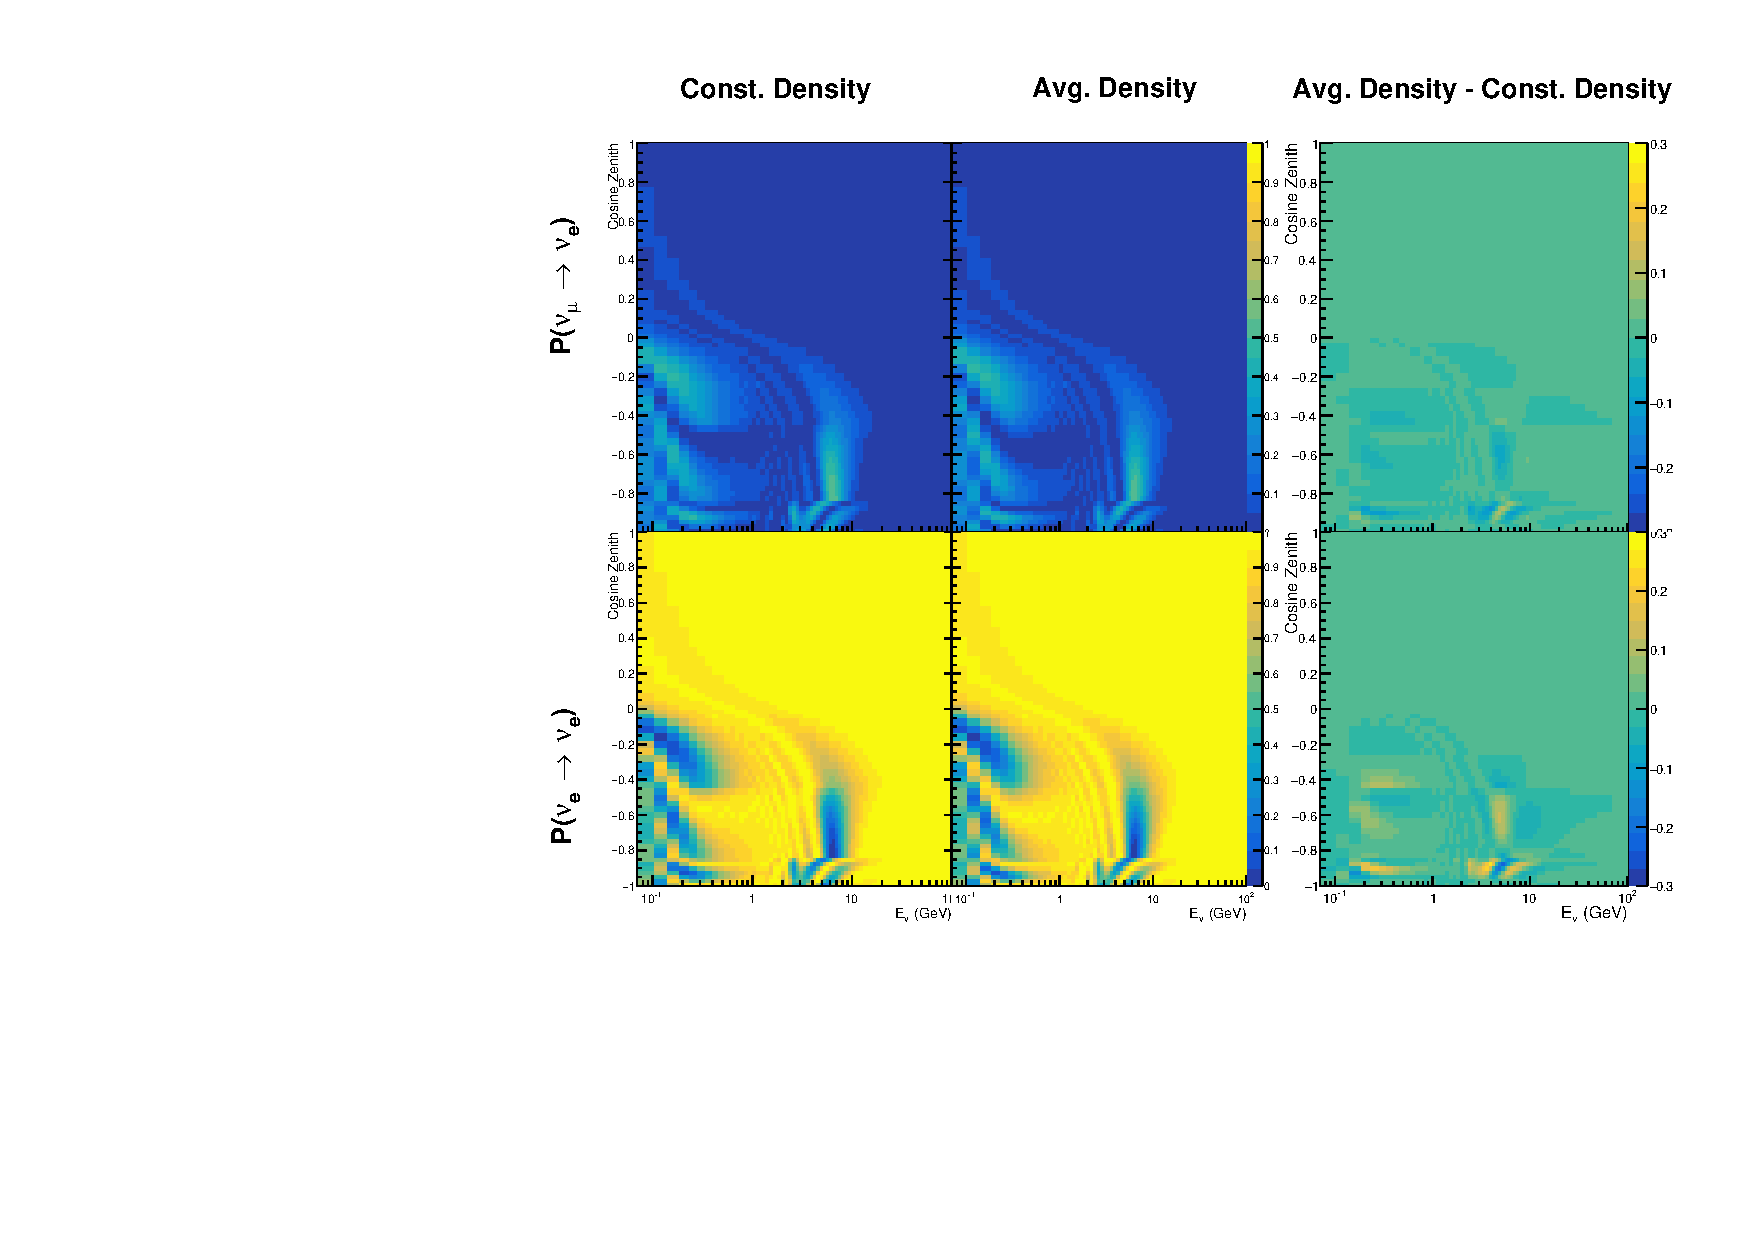
\includegraphics[width=\textwidth, trim={0mm 0mm 0mm 0mm}, clip,page=1]{Figures/Oscillation/AverageDensityPREMModel.pdf}
  \end{subfigure}
  \caption{The oscillation probability, \quickmath{P(\nu_{\mu} \rightarrow \nu_{e})} (top row) and \quickmath{P(\nu_{e} \rightarrow \nu_{e})} (bottom row), given as a function of neutrino energy and zenith angle. The left column gives probabilities where the four-layer constant density approximation is used. The middle column gives the probabilities where the density is integrated over the trajectory, using the quadratic PREM approximation, for each \quickmath{\cos(\theta_{Z})} is used. The right column illustrates the difference in oscillation probability between the two different techniques.}
  \label{fig:Oscillation_SK_AverageDensityPREMModel}
\end{figure}

\clearpage

\section{Production Height Averaging}
\label{sec:Oscillation_ProdHAvergaing}

As discussed in \autoref{sec:Oscillation_Overview}, the height at which the cosmic ray flux interacts in the atmosphere is not known on an event-by-event basis. The production height can vary from the Earth's surface to \quickmath{\sim50\text{km}} above that. The SK-only analysis methodology (described in \autoref{sec:Oscillation_FastOscillations}) for including the uncertainty on the production height is to include variations from the Honda model when pre-calculating the oscillation probabilities prior to the fit. This technique is not possible for this analysis which uses continuous oscillation parameters that can not be known prior to the fit. Consequently, an analytical averaging technique was developed in \cite{t2k_tn_425}. The author of this thesis was not responsible for the derivation of the technique but has performed the implementation and validation of the technique for this analysis alone.

\finish{Make sure the below paragraph clearly explains the variables used}
Using the \quickmath{20} production heights per Monte Carlo neutrino event, provided as \quickmath{5\%} percentiles from the Honda flux model, a production height distribution \quickmath{p_{j}(h | E_{\nu}, \cos{\theta_{Z}})} is built for each neutrino flavour \quickmath{j = {\nu_{e}, \bar{\nu}_{e}, \nu_{\mu}, \bar{\nu}_{\mu}}}. In practice, a histogram is filled with \quickmath{20} evenly spaced bins in production height \quickmath{h} between \quickmath{0} and \quickmath{50\text{km}}. The neutrino energy and cosine zenith binning of the histogram are the same as that provided in \autoref{sec:Oscillation_FastOscillations}. The average production height, \quickmath{\bar{h} = \int dh \frac{1}{4} \sum_{j} p_{j}(h | E_{\nu}, \cos(\theta_{Z}))}, is calculated. This assumes a linear average over the four flavours of neutrino which are considered to be generated in cosmic ray showers. The production height binning of this histogram is then translated into \quickmath{\delta t(h) = t(\bar{h}) - t(h)}, where \quickmath{t(h)} is the distance travelled along the trajectory.

\iffalse
Using the path length distributions from the Honda flux, the production height can be calculated via,
\begin{equation}
  h = \sqrt{L^{2} + 2LR_{SK} \cos(\theta_{Z}) + R_{SK}^{2}} - R_{Earth}
\end{equation}
where \quickmath{L} is the path length provided from the Honda flux model and \quickmath{R_{SK} = R_{Earth} + 380\text{m}} is the elevation of the SK detector.
\fi

For the \quickmath{i^{th}} traversed layer, the transition amplitude, \quickmath{D_{i}(t_{i+1},t_{i})}, is computed. The time-ordered product of these is then used as the overall transition amplitude via

\begin{equation}
  \label{eq:Oscillation_FullTransitionAmplitude}
  A(t_{n+1},t_{0}) = D_{n}(t_{n+1},t_{n})...D_{1}(t_{2},t_{1})D_{0}(t_{1},t_{0}),
\end{equation}

where,

\begin{equation}
  \label{eq:Oscillation_LayerTransitionAmplitude}
  \begin{split}
    D_{n}(t_{n+1},t_{n}) &= \exp[-i H_{n}(t_{n+1} - t_{n})] \\
    &= \sum^{3}_{k=1} C_{k} \exp[ia_{k} (t_{n+1} - t_{n})]
    \end{split}
\end{equation}

is expressed as a diagonalised time-dependent solution to the Schrodinger equation. The \quickmath{0^{th}} layer is the propagation through the atmosphere and is the only term that depends on the production height. Using the substitution \quickmath{t_{0} = t(\bar{h}) - \delta t(h)}, it can be shown that

\begin{equation}
  D_{0}(t_{1},t_{0}) = D_{0}(t_{1},\bar{h})D_{0}(\delta t).
\end{equation}  

\iffalse
\begin{equation}
  U_{n}(t_{n+1},t_{n}) &= \exp[-i H_{n}(t_{n+1} - t_{n})] , \\
  &= V \exp[-i A (t_{n+1} - t_{n})] V , \\
  H &= \sum_{k} u(k) a(k) u(k)^{\dagger}, \\
  V &= u \text{i.e. eigenvector} \\
  A &= a \text{i.e. diagonal} \\
  H &= V A V^{\dagger}, \\
  U_{0}(t_{n+1},t_{n}) &= V \exp[-i A (t_{n+1} - t_{n})] V^{\dagger}, \\
  U_{0}(t_{1},t_{0}) &= U_{n}(t_{1},\bar{h}-\delta t),\\
  &= V \exp[-i A (t_{1} - (\bar{h} - \delta t))] V^{\dagger}, \\
  &= V \exp-[i A (t_{1} - \bar{h})] \exp[i A \delta t))] V^{\dagger}, \\
  &= V \exp-[i A (t_{1} - \bar{h})] V^{\dagger} V \exp[i A \delta t))] V^{\dagger}, \\
  &= U(t_{1},\bar{h}) U(\delta t), \\
  V^{\dagger} V &= 1, \\
\end{equation}
\fi

Thus \autoref{eq:Oscillation_FullTransitionAmplitude} becomes

\begin{equation}
  \begin{split}
    A(t_{n+1},t_{0}) &= D_{n}(t_{n+1},t_{n})...D_{1}(t_{2},t_{1})D_{0}(t_{1},\bar{h})D(\delta t) \\
    &= A(t_{n+1},\bar{h}) \sum_{k=1}^{3} C_{k} \exp[ia_{k} \delta t], \\
    &= \sum_{k=1}^{3} B_{k} \exp[ia_{k} \delta t].
  \end{split}
\end{equation}

The oscillation probability averaged over production height is then calculated as

\begin{equation}
  \begin{split}
    \overline P(\nu_{j} \rightarrow \nu_{i}) &= \int d(\delta t) p_{j}(\delta t|E_{\nu}, \cos\theta_{Z}) P(\nu_{j} \rightarrow \nu_{i}) \\
    &= \int d(\delta t) p_{j}(\delta t|E_{\nu}, \cos\theta_{Z})	A(t_{n+1},t_{0}) A^{*}(t_{n+1},t_{0}) \\
    &= \sum_{km} (B_{k})_{ij} (B_{m})^{*}_{ij} \int d(\delta t) p_{j}(\delta t|E_{\nu}, \cos\theta_{Z}) \exp[i(a_{k}-a_{m})\delta t].
  \end{split}
\end{equation}

It is important to note that the exact value of \quickmath{\bar{h}} used does not matter as the values of \quickmath{\delta t} would change to compensate for any modification to the value of \quickmath{\bar{h}}.

In practice, implementation in CUDAProb3 \cite{cudaprob3} is relatively straightforward as the majority of these terms are already calculated in the standard oscillation calculation. \autoref{fig:Oscillation_SK_ProductionHeightAveraging} illustrates the results of the production height averaging. As expected, the main effect is observed in the low-energy downward-going and horizontal-going events. Upward-going events have to travel the radius of the Earth, \quickmath{R_{E} = 6371\text{km}}, where the production height uncertainty is a small fraction of the total path length. 

\begin{figure}[h]
  \begin{subfigure}[t]{\textwidth}
    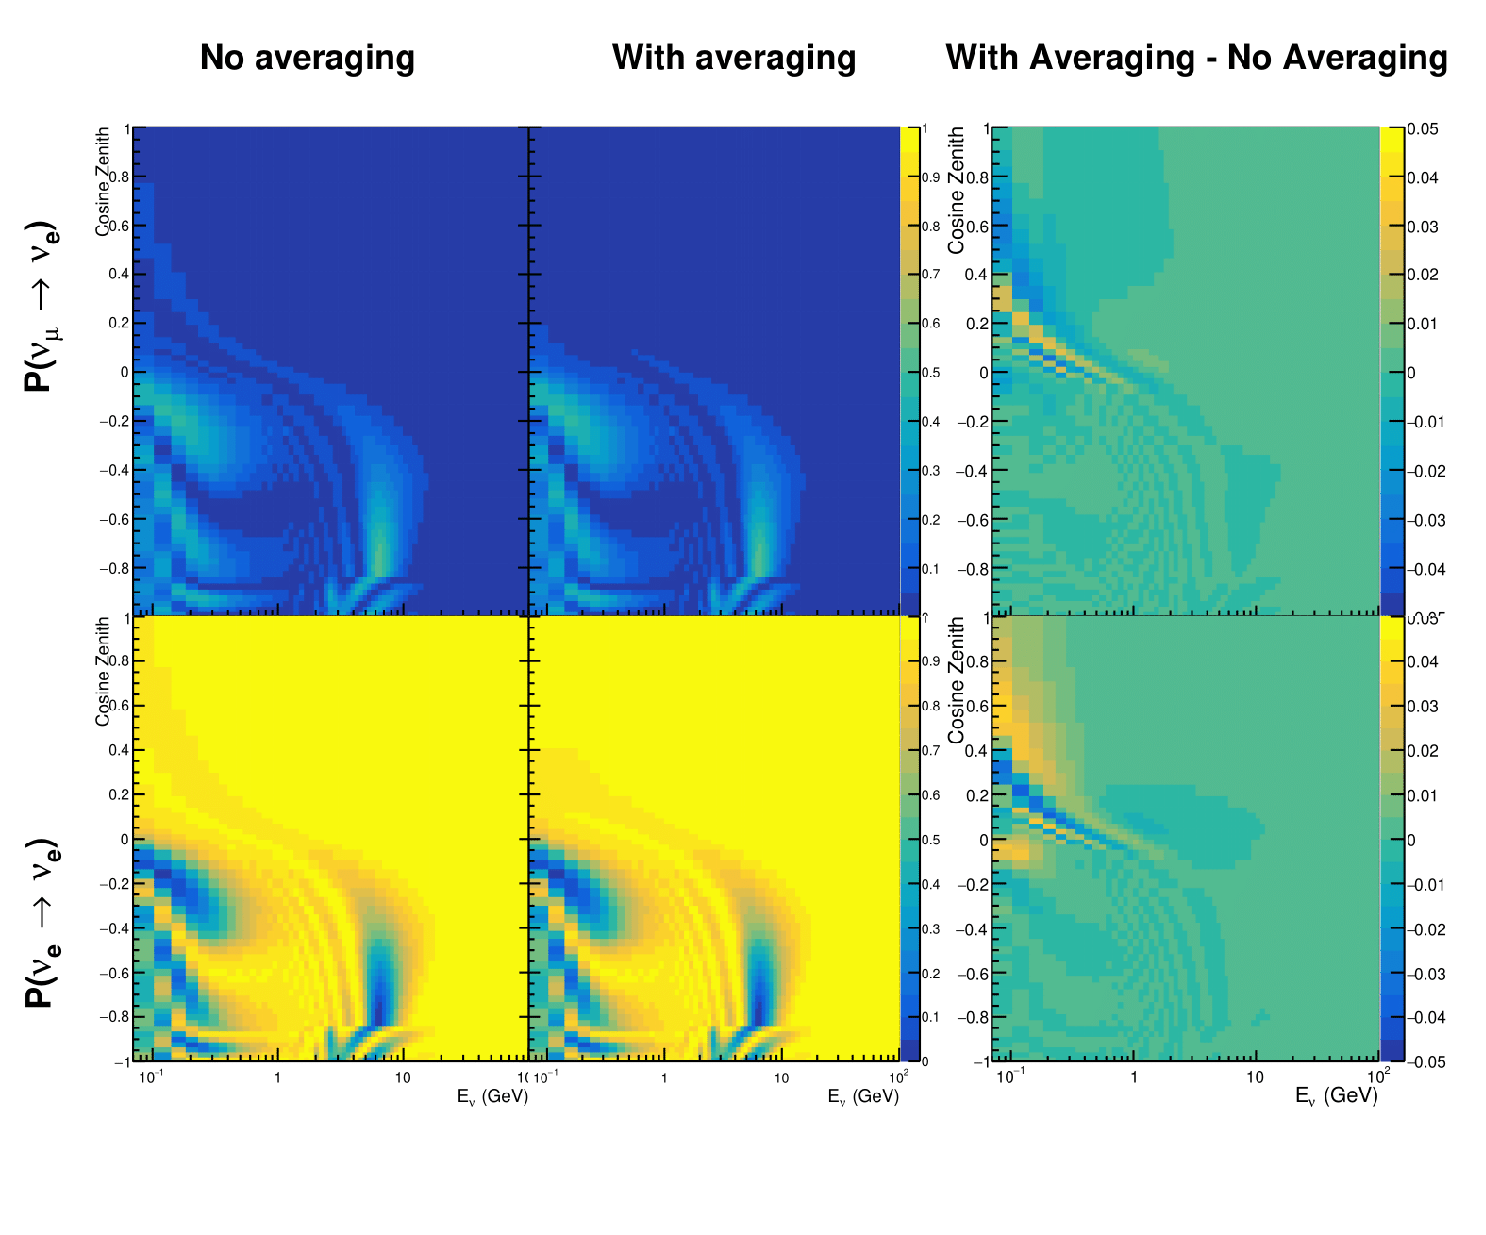
\includegraphics[width=\textwidth, trim={0mm 0mm 0mm 0mm}, clip,page=1]{Figures/Oscillation/ProductionHeightAveraging.pdf}
  \end{subfigure}
  \caption{The oscillation probability, \quickmath{P(\nu_{\mu} \rightarrow \nu_{e})} (top row) and \quickmath{P(\nu_{e} \rightarrow \nu_{e})} (bottom row), given as a function of neutrino energy and zenith angle. The left column gives probabilities where a fixed production height of \quickmath{25\text{km}} is used. The middle column gives the probabilities where the production height is analytically averaged. The right column illustrates the difference in oscillation probability between the two different techniques.}
  \label{fig:Oscillation_SK_ProductionHeightAveraging}
\end{figure}
